\chapter{Implementation}

\section{Review of design diagrams}
    \subsection{Entities diagrams}
    This diagram includes all properties and methods from every class in the app. It also contains enums and the navigation between the entities. \\
    As this diagram is too big to include it on the document, see it \href{https://github.com/JesusGonzalezA/LearnASLDoc/blob/master/doc/assets/diagrams/interfaces.png}{here}.

    \subsection{Interfaces diagrams}
    This diagram includes the definitions of all the interfaces in the application and the navigation between them. \\
    As this diagram is too big to include it on the document, see it \href{https://github.com/JesusGonzalezA/LearnASLDoc/blob/master/doc/assets/diagrams/entities.png}{here}.

    \subsection{Abstract factory to generate the questions}
    Due to maintenance reasons I opted to use this pattern to generate the questions. Imagine that, in the future, I want to add a new type of test. \\
    I should change all the logic in order to create just the questions for this test. \\
    As every question needs the same arguments in order to be created, just by using this pattern I would need to add a new question and factory. 
        \newpage
        \begin{figure}[H]
            \centering
                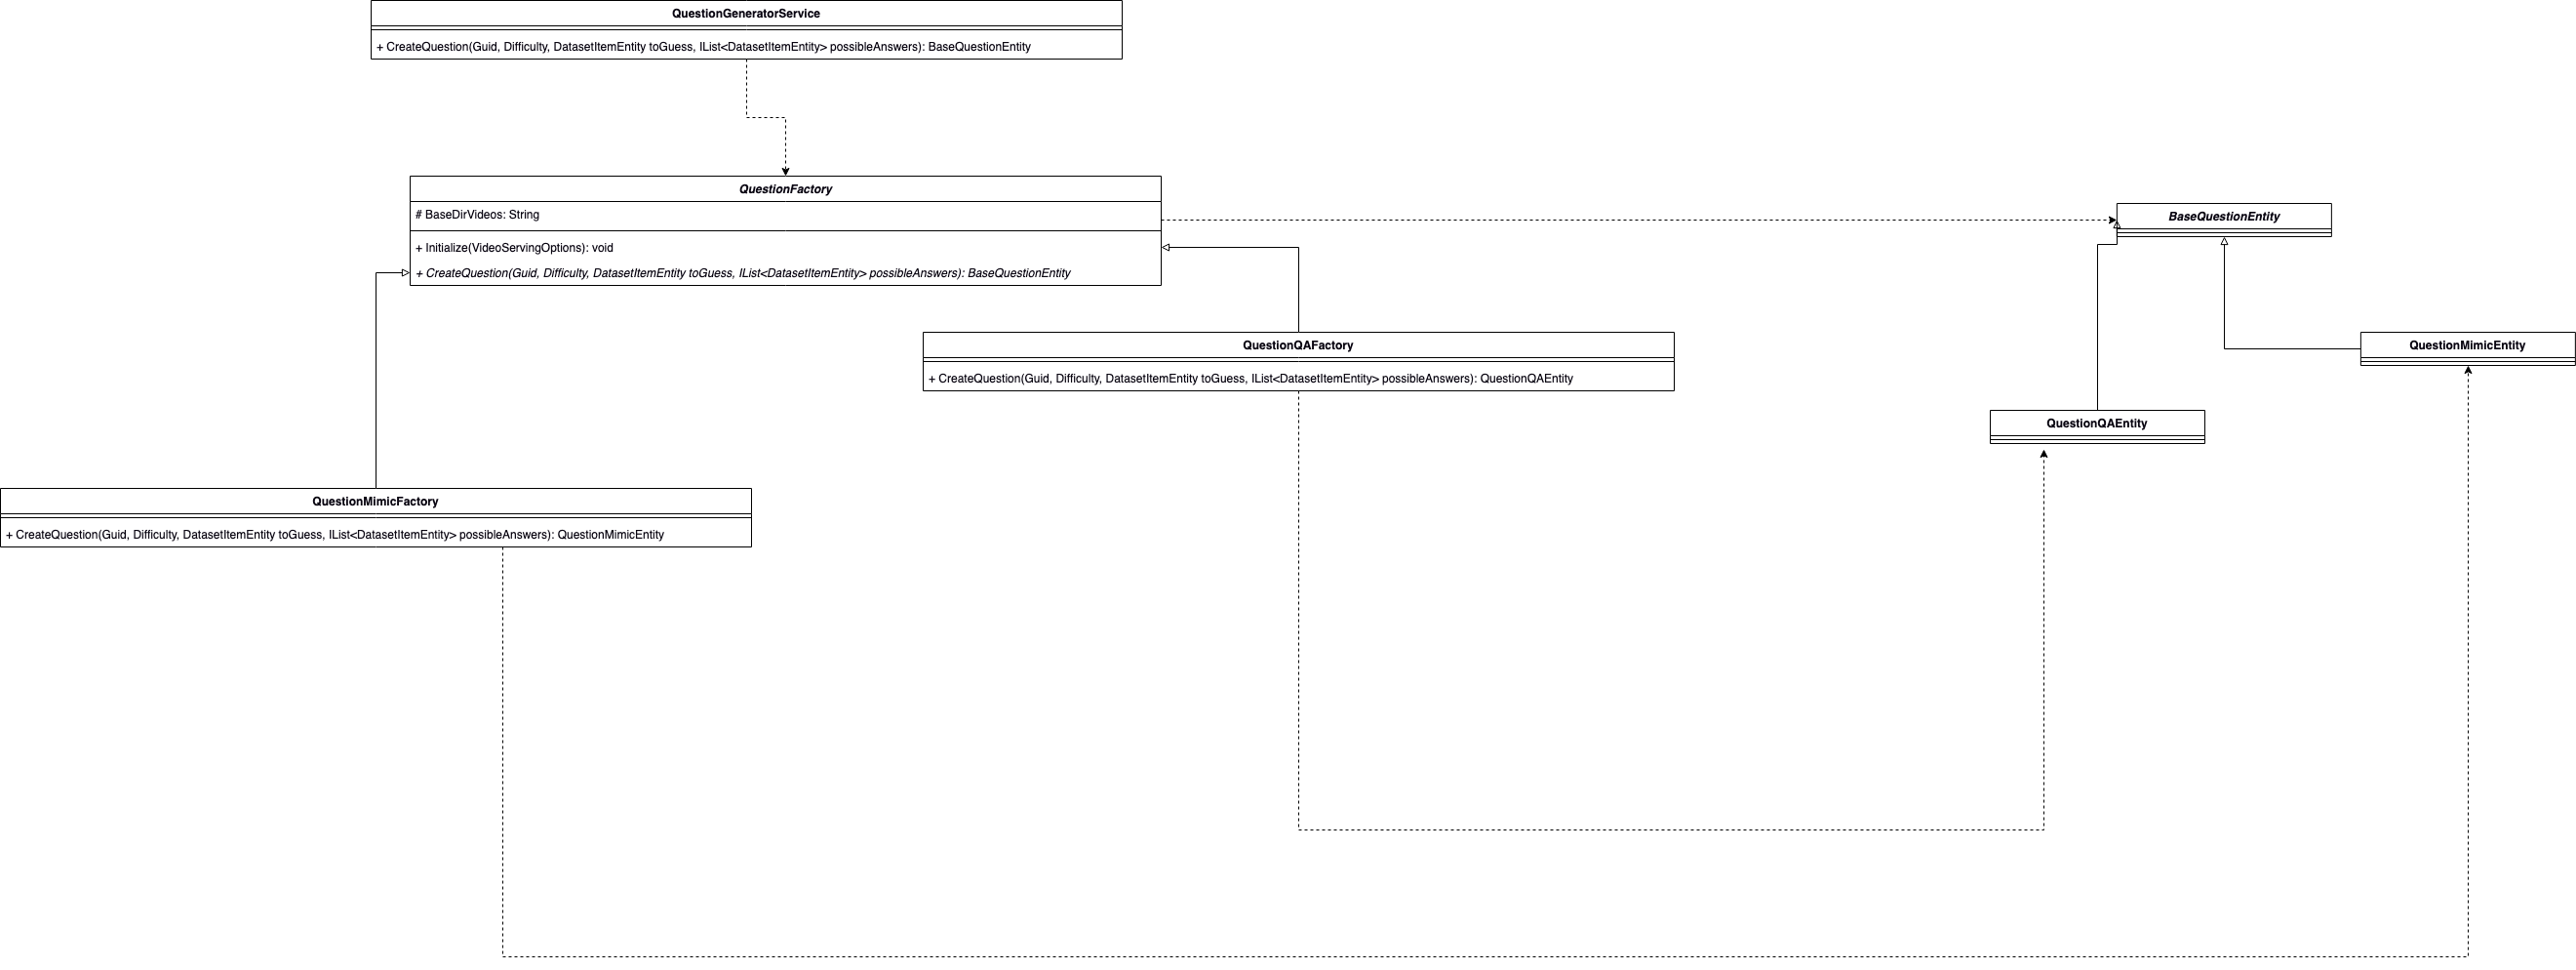
\includegraphics[angle=90, width=\textwidth, height=\textheight]{assets/diagrams/abstractfactory.png}
            \caption{Abstract factory}
            \label{fig:implementation_af}
        \end{figure}

\newpage
\section{Backend code documentation}
    \subsection{Architecture}
        \subsubsection{From MVC to Onion Architecture}
        \textbf{Model View Controller} (MVC) is the most commonly used web application architecture. It solves the separation of concern as there is a separation between \textit{View} (in this particular case the HTTP API responses), the \textit{Controller} (on which the business logic is added) and the \textit{Model} (it includes the database access).

        As we can see, we reach loose coupling, but tight coupling is still present. This is because classes are still dependent on concrete dependencies. \\

        \begin{figure}[H]
            \centering
                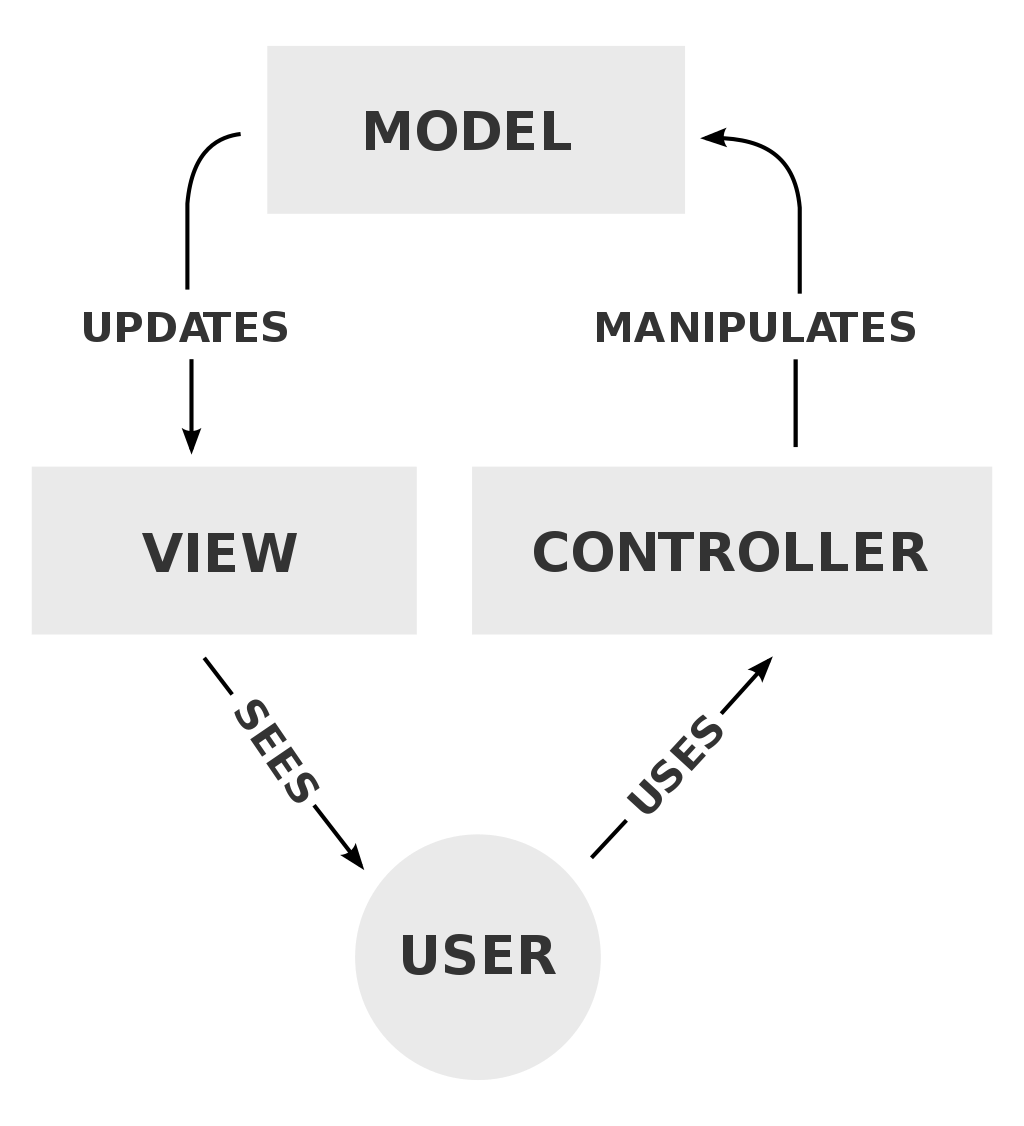
\includegraphics[width=0.5\textwidth]{assets/mvc.png}
            \caption{MVC \cite{MVC}}
            \label{fig:implementation_mvc}
        \end{figure}

        The \textbf{Onion Architecture} is very similar to \textit{MVC} because it keeps the separation of concerns but it solves the issue of tight coupling.

        \paragraph \textbf{How Onion architecture solves tight coupling?} \\
        It is based on Dependency Inversion Principle. All layers communicate with each other using interfaces. Concrete implementations are resolved on runtime. \\

        Layers are built on interfaces. This is also very convenient for testing purposes, due to the ease of exchanging a layer for a mock or another implementation object. \\
        The layers can change, but the idea is that all layers are towards to center, where the Core of the application is. It represents the business and behavior objects. \\

        \begin{figure}[H]
            \centering
                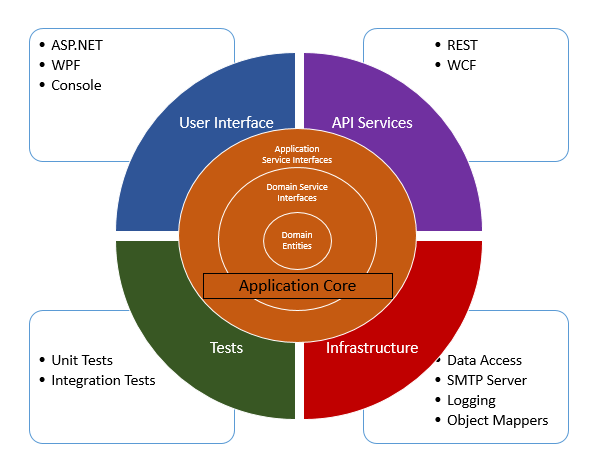
\includegraphics[width=\textwidth]{assets/onion.png}
            \caption{MVC \cite{OnionArchitecture}}
            \label{fig:implementation_onion}
        \end{figure}

        \subsubsection{How to orgnanize the project}
        \begin{itemize}[noitemsep]
            \item Test: it is used for testing purposes.
                \begin{itemize}[noitemsep]
                    \item References: all other layers.
                    \item Dependencies: xUnit.
                \end{itemize}
            \item Api: it is similar to view layer. It is the layer that will allow a client to interact with the application.
                \begin{itemize}[noitemsep]
                   \item Reponsabilities (as directories):
                        \begin{itemize}[noitemsep]
                            \item Controllers: define all the endpoints of the application and call the correct services on each method.
                            \item Middleware: catch users' calls to the Api. It allow to have a global exception handling, authorization, authentication...
                            \item Properties: define the launch settings for the Http Server.
                        \end{itemize}
                    \item References: Core
                    \item Dependencies:
                        \begin{itemize}[noitemsep]
                            \item Api Rest: Asp.Net Core 5.0
                            \item Documentation: Swagger
                        \end{itemize}
                \end{itemize}
            \item Core: it is the center part of the architecture. It contains the definition of all the entities of the application, both contracts for the Api communication with the clients and the entities, both model and data access entities. It also contains all the interfaces which are used to communicate between the Api layer and the Infraestructure (Other authors separate this into a new layer: service layer). This contains all the business logic and works with the data source.
                \begin{itemize}[noitemsep] 
                    \item Responsabilities (as directories):
                        \begin{itemize}[noitemsep]
                            \item Contracts: instead of sending and receiving the entities in the Api, a good approach is to use DTO (Data Transfer Objects). This way, the user don't need to send the Id before creating an entity, we can avoid to send properties that may be confidential such as passwords and we can retrieve just the needed information.
                            \item CustomEntities: definition of application entities, such as metadata to send information about pagination in the api, pagination entity, etc
                            \item Entities: definition of data access models.
                            \item Enums
                            \item Exceptions: definition of custom exceptions.
                            \item Extensions: helper functions to improve code readability.
                            \item Interfaces: interfaces for repositories and services of the app.
                            \item Options: implementation of options pattern.
                            \item QueryFilters: filters for get Api methods.
                            \item Services: implementation of services to control de data access.
                            \item ValidationAttributes: attributes to validate models.
                        \end{itemize}
                    \item References: None
                    \item Dependencies: None
                \end{itemize}
            \item Infraestructure: concrete implementations of all the services needed by the app to work.
                \begin{itemize}[noitemsep]
                    \item Responsabilities (as directories):
                        \begin{itemize}[noitemsep]
                            \item Data: definition of the context and migrations.
                            \item Extensions: initialize all the services and dependency injection container.
                            \item Factories: to implement abstract factory pattern to initialize the questions.
                            \item Filters: add flux to validate the model in the Api.
                            \item Mappings: to convert an entity to a contract and reverse.
                            \item Migrations: database creation and updates.
                            \item Repositories: implementation of repositories and unit of work pattern.
                            \item Services: implementation of services based on external implementations. For instance: service to hash a password, send an email, create a JWT...
                            \item Validators: validation rules for the API filters to validate the model. For instance: email should be valid, password should have 'x' length, date should be greater than 'x'...
                        \end{itemize}
                    \item References: Core
                    \item Dependencies:
                        \begin{itemize}[noitemsep]
                            \item Mail client: MailKit
                            \item ORM: Entity Framework Core
                            \item Validations: Fluent Validation
                            \item Logging: Serilog
                            \item Authentication: JWT
                            \item Mappings: automapper
                        \end{itemize}
                \end{itemize}
        \end{itemize}

        \subsubsection{Dependency injection}
        As this is a big project, following good design principles and patterns is important for its correct development and later maintenance. \\

        As the \textbf{SOLID principles} dictate, avoid depending on concrete implementations is a good practice as the application and its services may change. \\
        Instead of using the concrete implementations we let this work for interfaces. This way, the code in the upper layers won't change if the concrete implementation does, as the method signatures won't change. \\

        In ASP.NET it is recommended to use a dependency injection container and inject the dependencies in the constructor \cite{DI}. This way, the dependency injection container will change the interfaces for the concrete implementations and they will be passed automatically to the constructor. Let's see an example. \\

        In the next fragment of code, we can see how to configure the dependency injection container. This configuration corresponds to the \textit{Setup} class of the application. More concretely, it corresponds to the \textit{ConfigureServices} method, which receives an object that fits the \textit{IServicesCollection's interface} as an argument. \\
        This interface has the following methods to configure the dependency injection: \textit{AddTransient<Interface, Implementation>()}, \textit{AddSingleton<Interface, Implementation>()}, \textit{AddScoped<Interface, Implementation>()}. \\
        As we can notice, we can see a pattern: \textit{Add{LIFETIME}<{INTERFACE}, {IMPLEMENTATION}>()}. I'll talk about lifetime later on. \\

        The important thing here is that using these methods, the dependency injection container will know which object corresponds to every interface, so that we don't need to instanciate any object, the framework will do it for us. \\
        
        \lstinputlisting[language=CSharp, captionpos=t,
            caption={Dependency injection configuration}, 
            label={lst:impl_di_config}]
        {code/DependencyInjectionConfig.cs}
        

        In order to use these services, we can pass them through the constructor. We will have access only to the defined methods in the interface. The framework will automatically instanciate the object sending the correct object in the constructor. \\
        \lstinputlisting[language=CSharp, captionpos=t,
            caption={Dependency injection usage}, 
            label={lst:impl_di_usage}]
        {code/DependencyInjectionUsage.cs}
    

            \paragraph{Lifetime of an object}
            \begin{itemize}[noitemsep]
                \item \textbf{Transient:} services are created each time they're requested. Best for lightweight, stateless services.
                \item \textbf{Scoped:} services are created once per client request (connection). Better option when you want to maintain state within a request.
                \item \textbf{Singleton:} services are created the first time they're requested.
            \end{itemize}

    \subsection{Defining environment variables and storing secrets}
    As the application grows, it is important to use environment variables. It is good to separate the app into multiple environments, so you can test, build and develop in separate contexts. \\
    Using environment variables you avoid to define global constants in the code, so you can change the behaviour of the application without compiling the whole app. It is also a good practice because you separate it \\
    correctly. \\
    
    But, when you think of storing all the configuration globals of the application you can get into a trap. You can define private information in these files, but this information should not be visible \\
    to all members in the team, it should not be uploaded into repositories and it should be encrypted. \\

    In this subsection, we'll see how the \textit{options pattern} resolves a way to manage all these fields. Also, we'll see how to store this secret information in a development environment and what to use in production. \\

        \subsubsection{Options pattern}
        In the next fragment of code we can see an usage of this pattern. First, I define the options themselves. For instance, I defined options to configure the pagination. Another examples of options could be the neccessary information to build an \\
        email client, such as username, client id, password or secret... \\
        
        After defining the structure of the options, we should tell the framework how and from where get the options. In this case, I defined the options in a JSON file to configure the app called \textit{appsettings.json}. \\
        Other options are defined in the secrets or could be defined in other environments, even on cloud. This way you can hide your secrets and avoid uploading these to repositories or to encrypt the secrets. \\

        Finally, to use the secrets you just need to resolve the interface. This will be done automatically using dependency injection containers in ASP.NET.
            \lstinputlisting[language=CSharp, captionpos=t,
                caption={Options}, 
                label={lst:impl_options}]
            {code/Options.cs}
        \subsubsection{Microsoft's development implementation: User secrets}
        See \href{https://docs.microsoft.com/en-us/aspnet/core/security/app-secrets?view=aspnetcore-5.0&tabs=windows}{here} for more information. Every piece of sensitive data is considered a secret. In order to store them in a safer way, we can use the \textit{Secret Manager Tool} provided by \textit{Microsoft}. \\
        The values are stored in a JSON file in the local machine. Due to this, it is not safe in a production environment as it is not encrypted. \\
        To make easier this task, I created the structure of all the secrets to configure in the app. This is the next code fragment. After modifying the JSON file with the correct information and just typing the commands in the next code fragment all the user secrets in the app will be correctly configured. \\

        \lstinputlisting[escapechar=+, language=json, captionpos=t,
            caption={JSON containing the definition for the user secrets}, 
            label={lst:impl_user_secrets_input}]
        {code/secrets.json}

        \lstinputlisting[escapechar=+, language=bash, captionpos=t,
            caption={Init and configure user secrets}, 
            label={lst:impl_user_secrets}]
        {code/usersecrets.bash}

        \subsubsection{Moving into a production environment}
        For production cases, it is recommended to use other options that provide encrypted store of the secrets. A recommended way by Microsoft is \textbf{Azure Key Vault} \cite{AKV}

    \subsection{Using extension methods to clean startup method}
    As the services and the configuration grow in the application, the \textit{Startup} class becomes less maintenable. Also, it would be good to separate the configuration in multiple files, as the responsability is different and the reason of change. \\
    
    \lstinputlisting[escapechar=+, language=CSharp, captionpos=t,
        caption={Refactoring startup method}, 
        label={lst:impl_startup_refactor}]
    {code/StartupExtensions.cs}

    All code is moved to this extension class. Passing the \textit{this} keyword to a static method, you can add the method to the object definition. The rest of the arguments will be the new method's arguments. \\
    This way only this new class will change whenever a new service is added, so the repository will be cleaner. The services object is returned so that the methods can be chained.
    \lstinputlisting[language=CSharp, captionpos=t,
        caption={Service collection's extensions methods}, 
        label={lst:impl_startup_extensions_1}]
    {code/StartupExtensions1.cs}

    \subsection{Entity framework}
        \subsubsection{Code first}
        Following \textit{Donatas Kimutis}'s recommendations \cite{Kimutis}, I use this approach. Firstly, I define the classes and mappings in the code. Then, the databases are created from the code. All evolutions are made via migrations. \\
        If the work is from an existing database, there are tool for reversing engineering. \\

        To mark navigational properties, I use \textit{virtual} keyword. This also enables \textit{Lazy Loading}, so these entities are only loaded when used. \\

        In the next fragment of code we can see the \textbf{User entity}. A user has the following properties:
        \begin{itemize}[noitemsep]
            \item Email
            \item Password
            \item ConfirmedEmail
            \item TokenPasswordRecovery (optional)
            \item TokenEmailConfirmation (optional)
            \item Tests (navigation property). A user can have 0 or multiple tests.
        \end{itemize}

        \lstinputlisting[language=CSharp, captionpos=t,
            caption={User entity model creation}, 
            label={lst:impl_userentity}]
        {code/Virtual.cs}

        \subsubsection{Entity}
            In order to use generic repositories and track the events in the objects that will be stored in the database I need to create a base class. This class will be \textit{abstract}, as won't be instanciated. 
            
            \lstinputlisting[language=CSharp, captionpos=t,
                caption={Entity class}, 
                label={lst:impl_entity}]
            {code/Entity.cs}

        \subsubsection{Automatically tracking entities through events}
        When an operation with the database is made, the \textit{Entity framework} tracks the entity.  
        In the constructor of the \textit{DatabaseContext} class, I set up two methods to do when two events are fired. See \href{https://docs.microsoft.com/en-us/dotnet/api/microsoft.entityframeworkcore.changetracking.changetracker?view=efcore-5.0}{here}. \\

        When the event \textbf{StateChanged} is fired, the method \textit{OnEntityStateChanged} will be executed. It will update the parameter \textit{ModifiedOn} from the \textit{Entity} if the tracked entity is being modified.
        When the event \textbf{Tracked} is fired, the method \textit{OnEntityTracked} will be executed. It will update the parameter \textit{CreatedOn} from the \textit{Entity} if the tracked entity has been created.

            \lstinputlisting[language=CSharp, captionpos=t,
                caption={Entity tracking}, 
                label={lst:impl_entity_tracking}]
            {code/EntityTracking.cs}
        
        \subsubsection{Repository pattern}
            For this section, I used a guide from Microsoft \cite{RepoAndUW}. \\
            It is intended to add an abstraction layer between the data access and the business logic layer. To implement the repository pattern, I need to create an interface and an implementation for every entity in the application. \\
            As some functions are common for these entities, I can create a generic repository. \\

            In the next code fragment, I define the generic interface for the repositories. Note that the generic type \textit{T} should inherit from the \textit{BaseEntity}.
            \lstinputlisting[language=CSharp, captionpos=t,
                caption={Interface for the generic repository}, 
                label={lst:impl_ibaserepository}]
            {code/IBaseRepository.cs}

        \subsubsection{Unit of work pattern}
            For this section, I used a guide from Microsoft \cite{RepoAndUW}. \\
            As the application grows, more entities and repositories appear. The \textit{unit of work pattern} makes the use of these repositories cleaner and it ensures that all repositories share a single database context. \\

            \begin{figure}[H]
                \centering
                    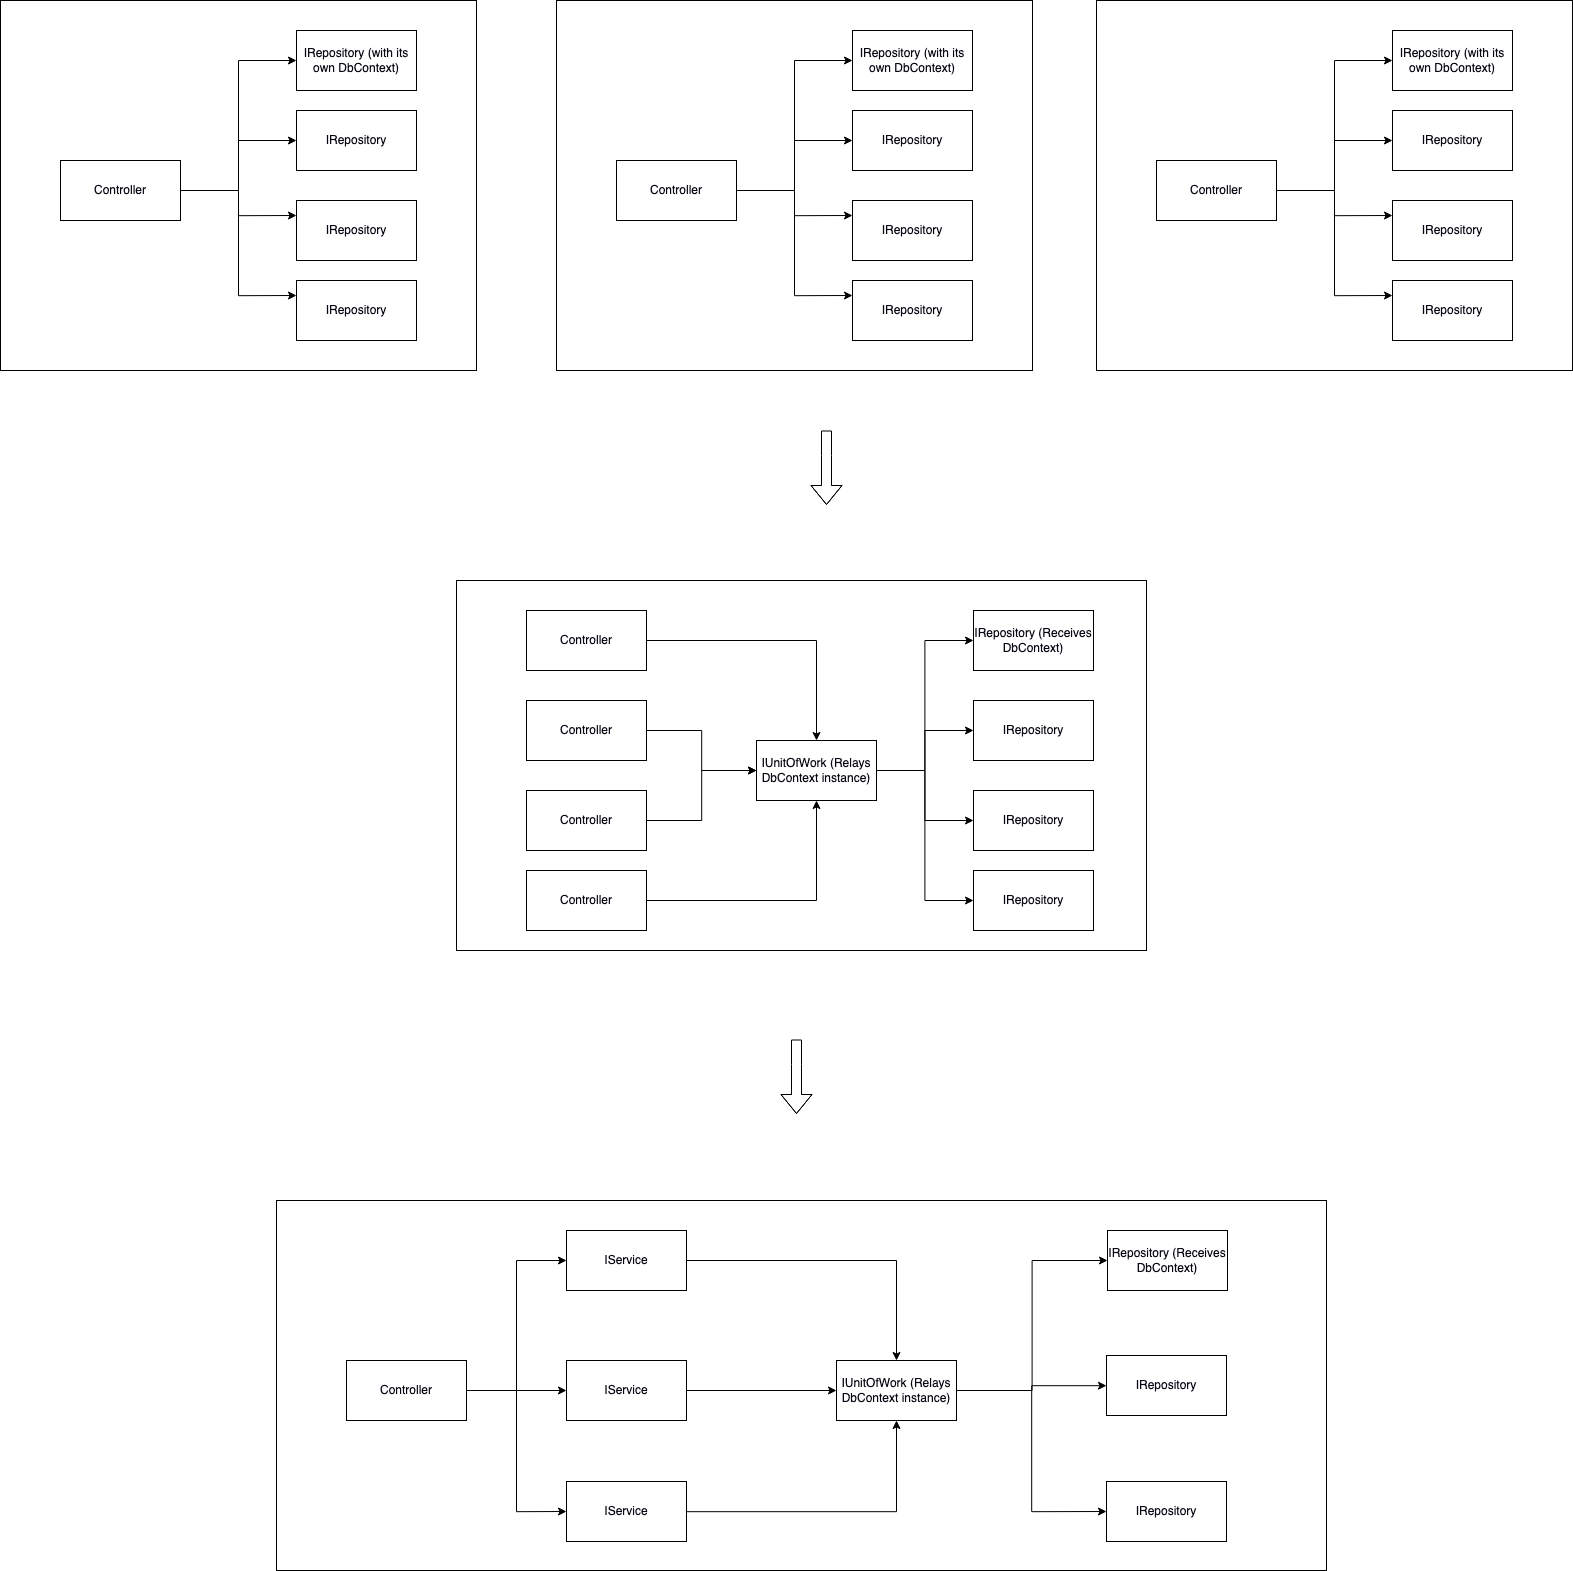
\includegraphics[width=0.9\textwidth]{assets/diagrams/unitofwork.png}
                \caption{Unit of Work}
                \label{fig:implementation_unit_work}
            \end{figure}
    
    \subsection{Error handling middleware}
    It is important to handle the errors of the application. Good reasons to do it could be to find errors in the code, send alerts if something has failed or stopped working, \\
    to avoid sending sensitive information to the client, etc. \\

    As we can see in the next code fragment, in the \textit{Startup} class I define the use of this middleware. \\
    The middleware capture the exceptions from the rest of middlewares and execution from the controllers. \\

    I catch all exceptions, although I do a separation: custom exceptions (\textit{BusinessExceptions} and \textit{ControllerExceptions}) and the rest. \\
    The custom exceptions are thrown by me, so I just send the error message to the client with a custom code. \\
    On the other hand, the rest of the exceptions are not handled by me. These could be network exceptions, from other dependencies such as the \textit{ORM}, etc. These exceptions are logged and \\
    the stack trace is sent to the client if the environment is set to \textit{Development}. \\
    \lstinputlisting[language=CSharp, captionpos=t,
        caption={Error handling middleware}, 
        label={lst:impl_ehm}]
    {code/ErrorHandlingMiddleware.cs}

        \subsubsection{Logger}
        All logs are saved in the \textit{Log} directory. The name of the file comes from the day. Every log entry contains the next information:
        \begin{itemize}[noitemsep]
            \item Date and hour
            \item HTTP method from the request
            \item Route of the request
            \item Stack trace
        \end{itemize}
        \begin{figure}[H]
            \centering
                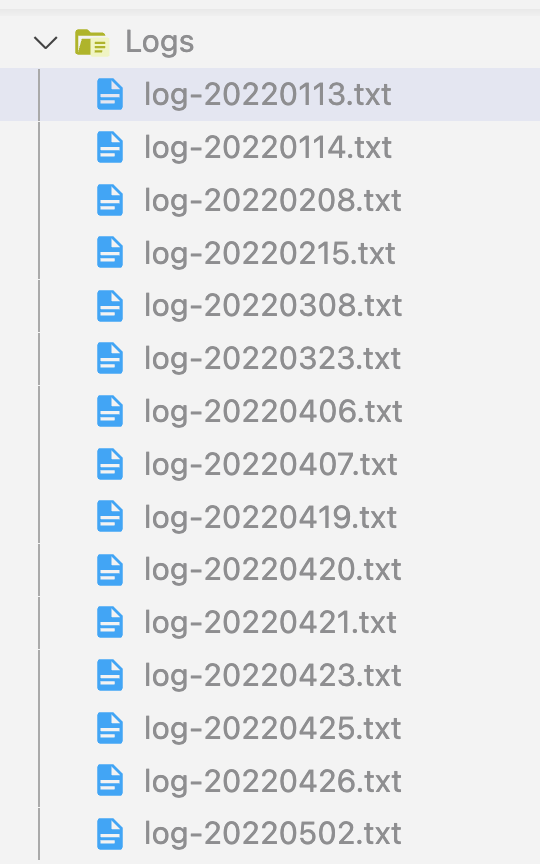
\includegraphics[width=0.3\textwidth]{assets/logs.png}
            \caption{Logs}
            \label{fig:implementation_logs}
        \end{figure}
        
    \subsection{Mapping}
        As Microsoft states \cite{DTO}, there are some cases in which you don't want to expose your database entities to the client in an \textit{API}. These cases could be:
        \begin{itemize}[noitemsep]
            \item Remove circular references
            \item Hide properties 
            \item Reduce payload size
            \item Populate nested objects 
            \item Protect sensitive data
            \item Decouple the service layer from the database layer
        \end{itemize}

        In conclusion, the data transfer object is an entity with all the data you need to send to the client. It is constructed from the database entity. Therefore, you should have methods to transform a \textit{DTO} to a \textit{Database object} and viceversa. This process is called \textbf{Mapping}.

        \subsubsection{AutoMapper}
        To make the mapping process easier, I used a library called \textit{AutoMapper} \cite{AutoMapper}. \\

        In the next code fragment, I show how to set up \textit{AutoMapper}. The first thing to do is creating a profile. In this case, I show a profile to map from \textit{UserDto} to \textit{UserEntity}, which is the database entity. Note that this map is reversible and, as both entities inherits from a base class, this class should have an own mapping too. The next thing to do is creating adding the profile to the \textit{mapper configuration} and setting up in the \textit{services}. Then, I can simply use it to map from an entity to the other. \\
        \lstinputlisting[language=CSharp, captionpos=t,
            caption={Mapping example}, 
            label={lst:impl_automapper}]
        {code/AutoMapper.cs}

    \subsection{Filters: automatic validation}
    According to Microsoft \cite{Filters}, filters allow to run code before or after specific stages in the request process pipeline. This specific filter, runs before the controller action and aims to avoid running unnecessary code due to the fact that the request is badly formed. \\

        \subsubsection{Using validators}
        I use a library called \textit{FluentValidation} \cite{FluentValidation}. This one allows a strongly-typed validation. \\

        In the next fragment code, I show how to create a new custom validator and set it up in the \textit{Startup} class. \\
        The class \textit{LoginDtoValidator} is a validator for the \textit{DTO} object \textit{LoginDto}. It adds rules for the object to not have an empty \textit{Email}, not having an empty \textit{Password} and its length from 6 to 15 and having a password that matches a \textit{RegEx} that checks if it has at least a lowercase and uppercase letter, if it has a digit and if it has at least a symbol. \\

        \lstinputlisting[language=CSharp, captionpos=t,
            caption={Configure the login dto validator}, 
            label={lst:impl_filtervalidator}]
        {code/Filters_Validator.cs}

        \subsubsection{Using attributes}
        They are called \textbf{Data annotations}. They serve the same thing, but it is less powerful, as they do not support conditional validations, they do not support validations in sets (check the field 'x' when the field 'y' is 'z'...). Nevertheless they are easy to use and they fulfill their purpose. \\
        For simple cases, such as the next one, I only use this type of validation. In the next code fragment I show how to create an attribute to check if the model is valid or not. It checks the length of a file. If it is bigger than the configured value, the model is incorrect.

        \lstinputlisting[language=CSharp, captionpos=t,
            caption={Configure an attribute to validate the max file of a file}, 
            label={lst:impl_filterattributes}]
        {code/Filters_attributes.cs}

    \subsection{Security}
        \subsubsection{Hashing passwords}
        As Microsoft recommends \cite{Hash}, I use \textbf{Pbkdf2 algorithm} to hash the passwords. It is a key derivation function to reduce brute-force attacks. \\

        The algorithm receives as arguments the \textit{password, salt and iterations}. It is important to think in the check process before hashing the password. \\
        In order to check the encrypted password, I would need the same arguments. If the salt or iterations varied from a password to another one, I should include this into the tuple in the database too. \\
        
        This way, every password could have a different salt and/or iterations. I would read the encrypted password, the salt and the iterations that I used to hash the password and I could check it this way. \\
        A way of doing it could be having this structure: \textit{<iterations>.<salt>.<encrypted\_key>}. \\
        
        The next fragment of code shows how to implement this. \\

        \lstinputlisting[language=CSharp, captionpos=t,
            caption={Method to hash a password}, 
            label={lst:impl_hash}]
        {code/PasswordService_Hash.cs}

        \begin{figure}[H]
            \centering
                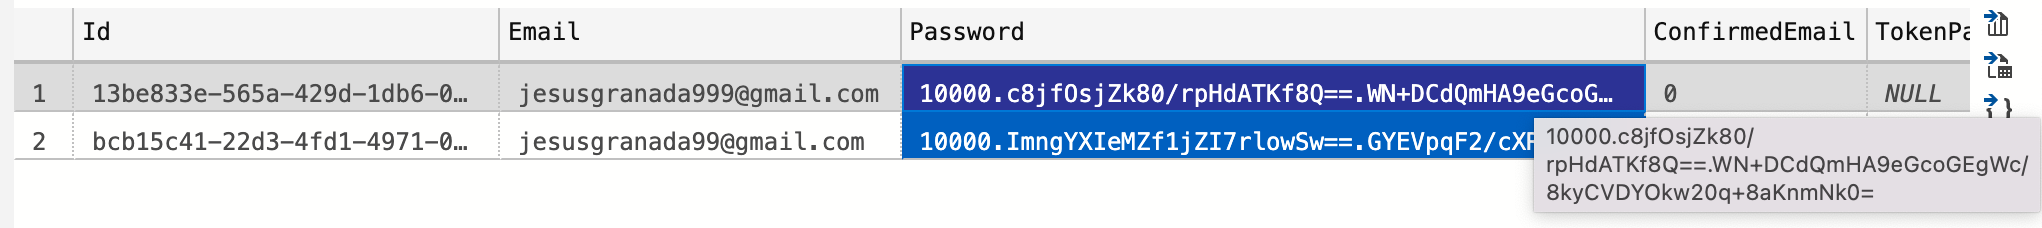
\includegraphics[width=0.9\textwidth]{assets/users_database.png}
            \caption{Encrypted passwords in the database}
            \label{fig:user_database}
        \end{figure}

        As I said before, the structure of the tuple in the database was \textit{<iterations>.<salt>.<encrypted\_key>}. This way, I could split the password from the database into three parts by the character '.'. \\

        The first part should be the number of iterations, the second one should be the salt and the third part the encrypted key. These would be the arguments to check the password. \\

        In the next fragment of code I show how to implement this. \\

        \lstinputlisting[language=CSharp, captionpos=t,
            caption={Method to check a password}, 
            label={lst:impl_password}]
        {code/PasswordService_Check.cs}

        \subsubsection{JWT tokens}
        A JWT (Json Web Token) \cite{JWT.io} is a standard way to share claims securely between two parties. The token is divided in three parts. Each part is divided by the character '.'. \\
        \begin{itemize}[noitemsep]
            \item The first part includes information about the algorithm and token type.
            \item The second part is the payload. It includes all the claims.
            \item The third part is the verify signature.
        \end{itemize}

        You should not include confidential information in the claims as they can be read. The thing is that, by signing this token, I can securely communicate with my API and identify the user. This way I can avoid having sessions. \\
        Also, the tokens has a issuing date. This way, you can check the date and only validate those signed before 'x' date. \\

        In order to communicate with the server, you need to include the \textit{Authorization} header in the HTTP request. The structure would be: \textit{Authorization: Bearer <your\_jwt>}. \\

        In the next figure, I show how to send a request to a protected route in the API. The response is unauthorized, as the token is invalid. \\
        \begin{figure}[H]
            \centering
                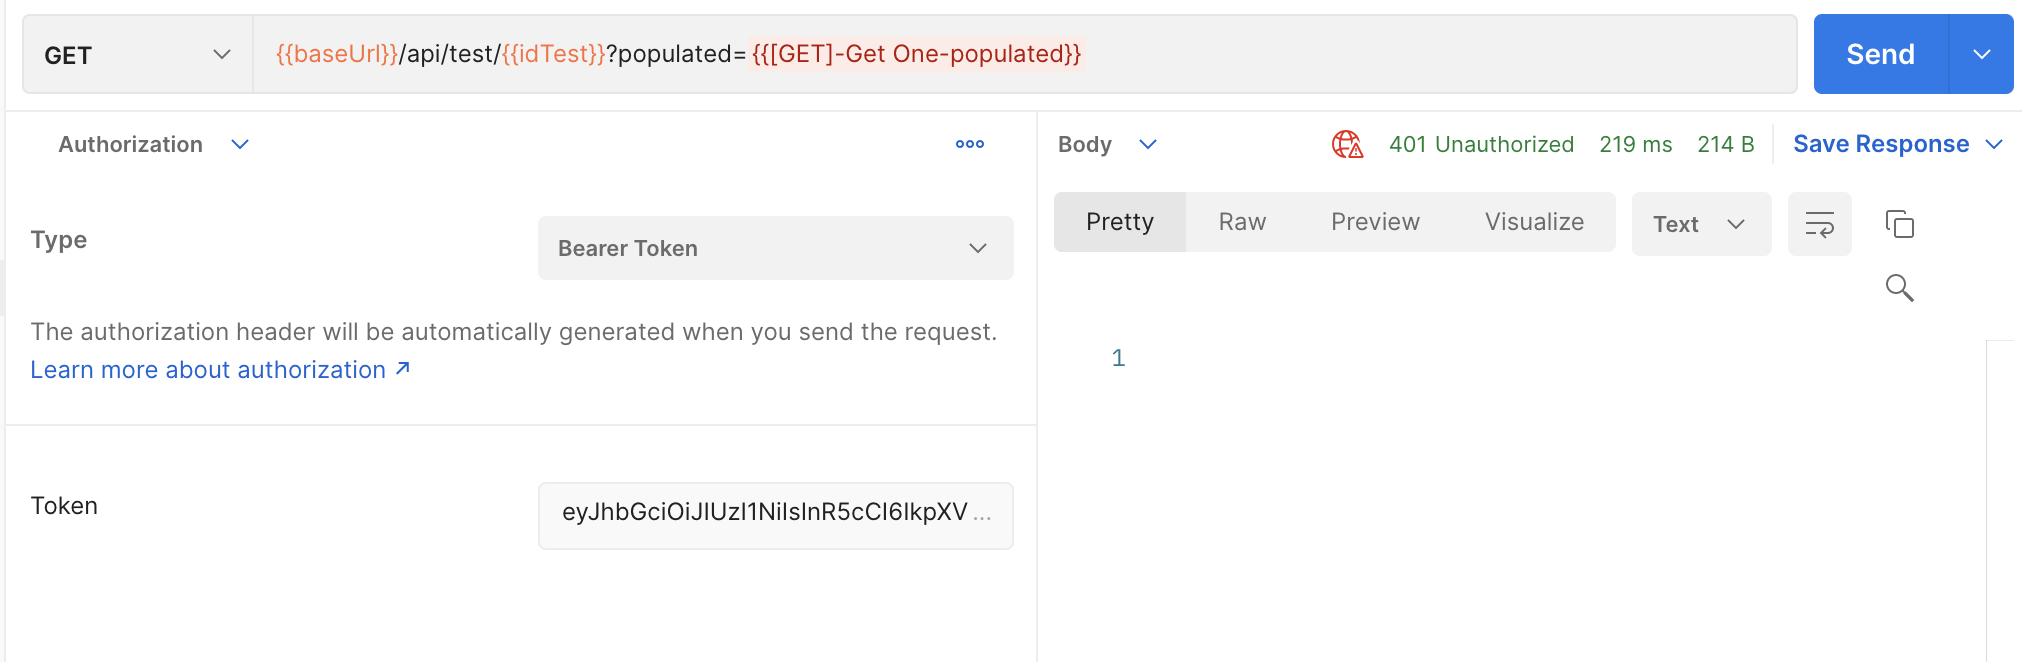
\includegraphics[width=0.9\textwidth]{assets/unauthorized.png}
            \caption{Unauthorized response}
            \label{fig:user_unauthorized}
        \end{figure}

        As the token is invalid, the user would have to login in the app to get access to a token. \\
        \begin{figure}[H]
            \centering
                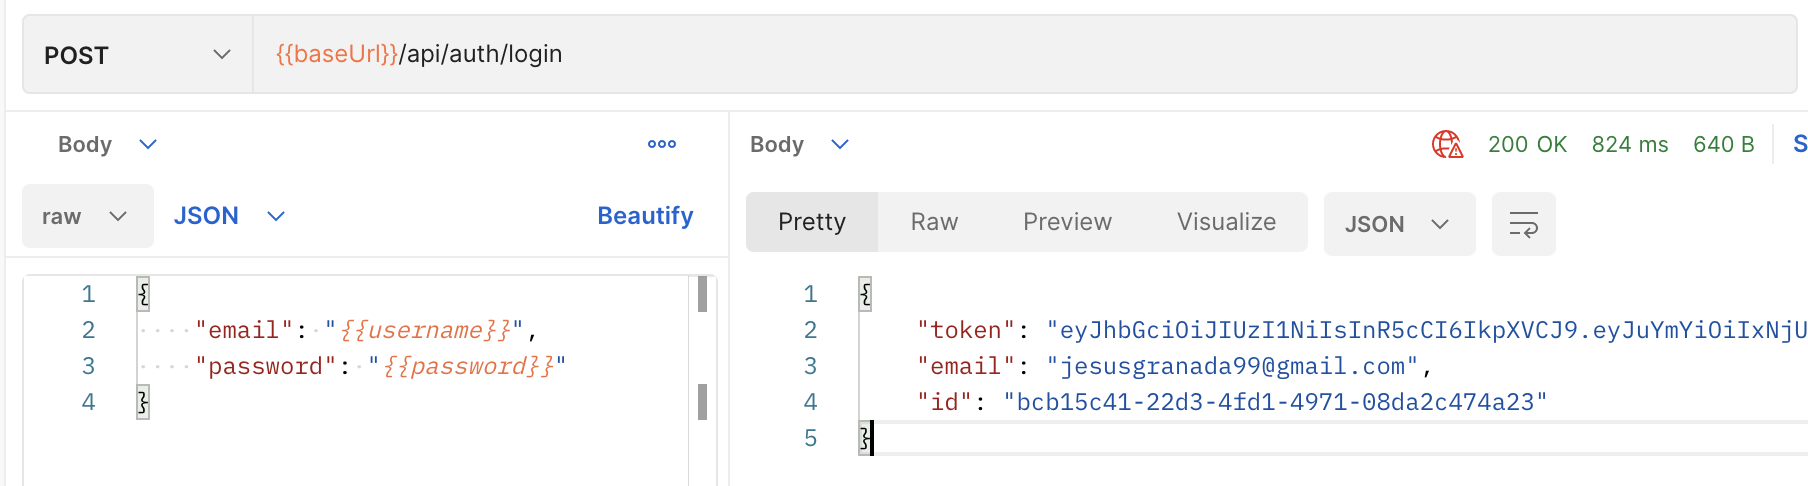
\includegraphics[width=0.9\textwidth]{assets/login.png}
            \caption{Login in the API}
            \label{fig:user_login_api}
        \end{figure}

        In the next figure, you can see the payload from the token. It has the following claims:
        \begin{itemize}[noitemsep]
            \item \textbf{nbf:} not valid before (seconds since Unix epoch).
            \item \textbf{exp:} expiration time (seconds since Unix epoch).
            \item \textbf{emailaddress:} email address of the user.
            \item \textbf{nameidentifier:} unique identifier.
        \end{itemize}
        \begin{figure}[H]
            \centering
                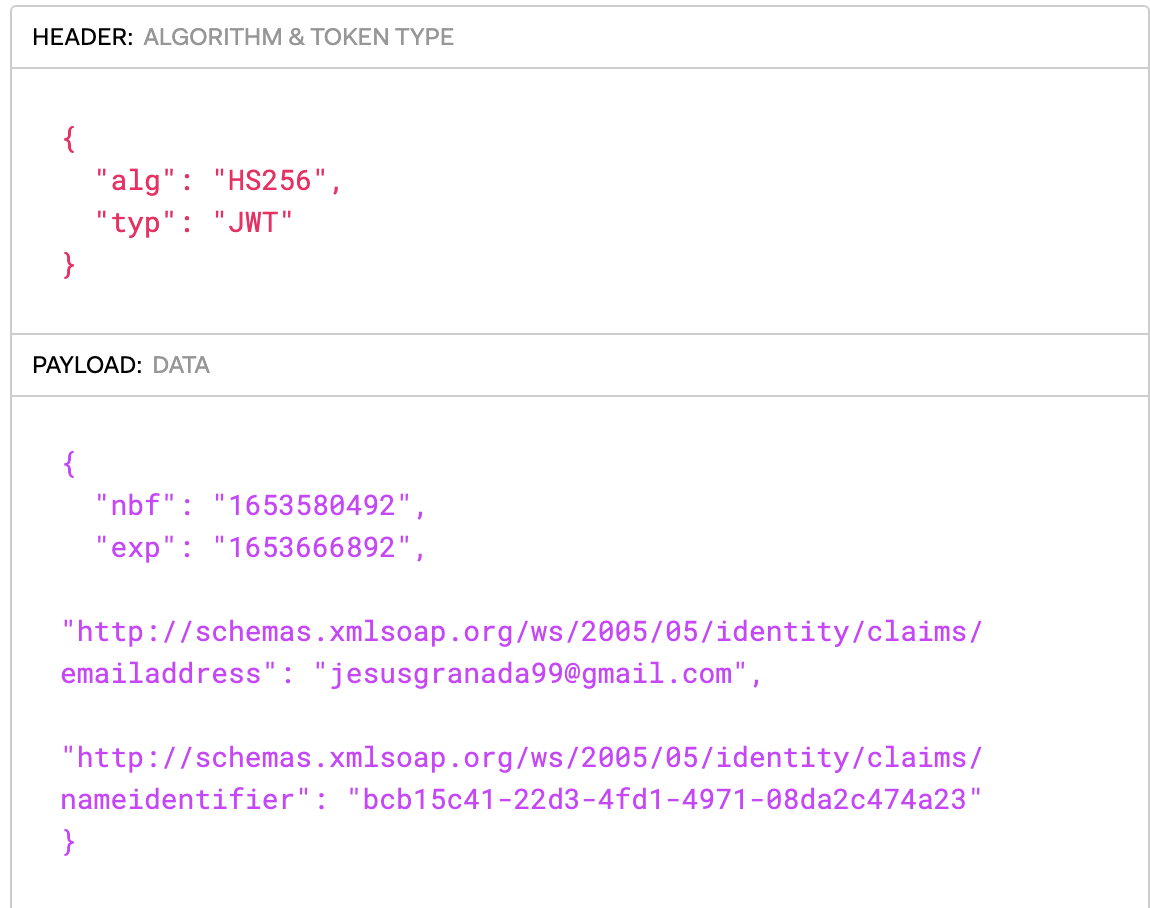
\includegraphics[width=0.9\textwidth]{assets/jwt.io.png}
            \caption{JWT claims}
            \label{fig:user_jwtclaims}
        \end{figure}

        Now the user can interact with the API as they have a correct token.
        \begin{figure}[H]
            \centering
                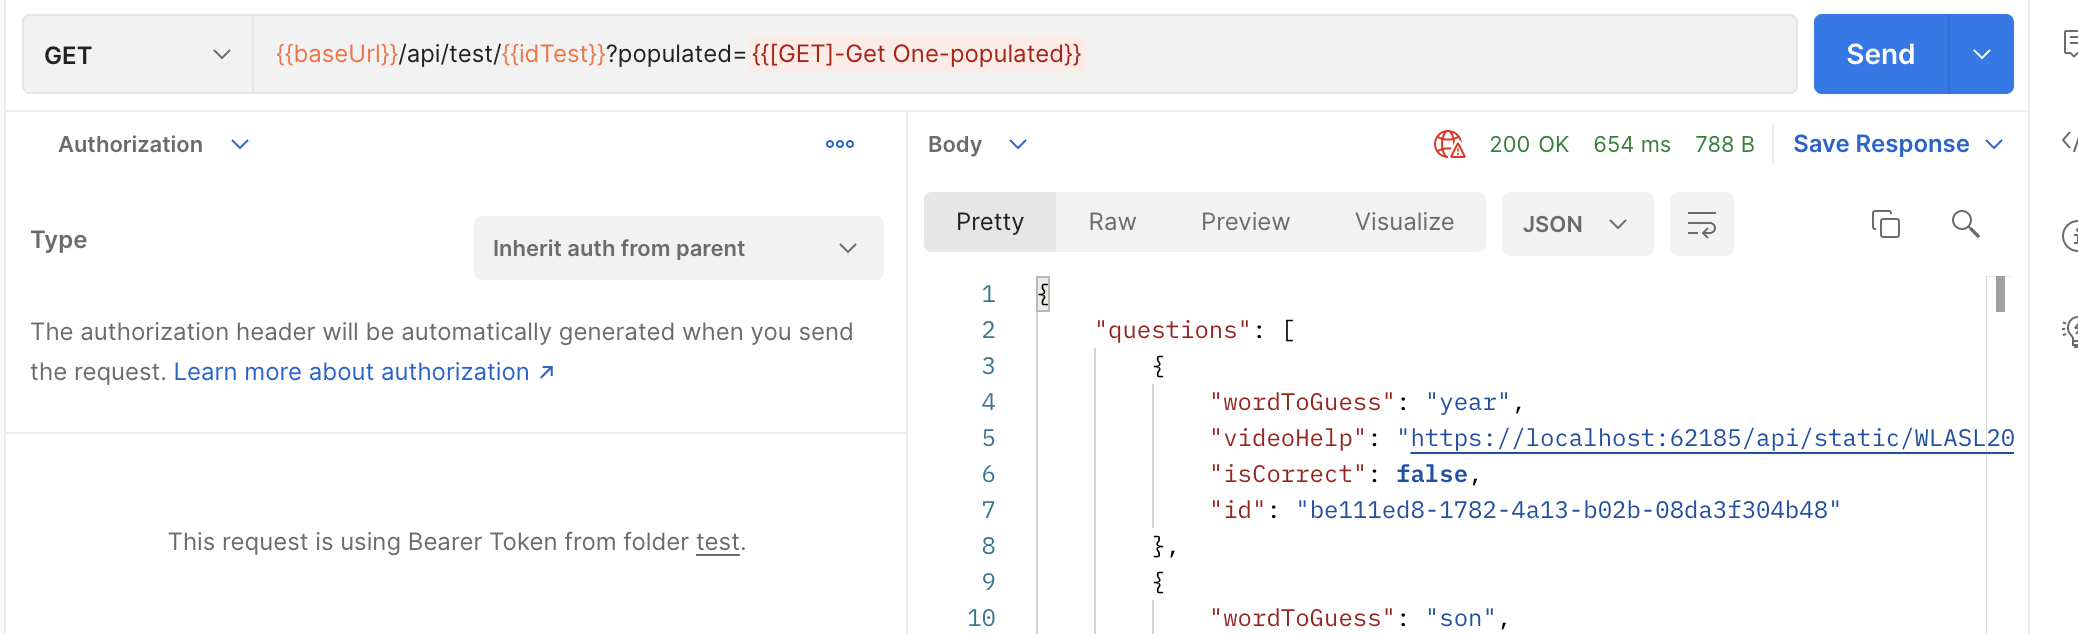
\includegraphics[width=0.9\textwidth]{assets/authorized.png}
            \caption{Authorized response}
            \label{fig:user_authorized}
        \end{figure}

        \subsubsection{Configuring CORS}
    As MDN indicates \cite{CORS}, CORS (Cross-Origin Resource Sharing) is an HTTP header mechanism that allow a server to indicate other than its own from which a browser should permit loading resources. \\
    Browsers do a \textit{preflight} request before doing the actual one to check if the server allows the request from this origin and this concrete method. \\

    In the next fragment of code, I show how to implement the CORS policy in the app. It allow any method from the frontend origin. \\
    \lstinputlisting[language=CSharp, captionpos=t,
            caption={Configuring CORS}, 
            label={lst:impl_cors}]
    {code/Cors.cs}

    \subsection{Email service}
    In order to register in the application, a requisite is to have a valid email account. This is because the account will be checked, \\
    so only real users with their real accounts will be registered. \\

    Also, this allows to recover a password easily from the email and, in future versions, create email lists. \\

    \subsubsection{Authorization flux}
    The process could have been done using \textit{SSO}, \textit{OAuth flux}... \\
    Nevertheless, I was recommended to use my own authorization flux in order to learn by my teachers in \textit{Vilnius University}. \\

    \paragraph{Registration flux}
    This way, the flux of registration would be the following:
    \begin{enumerate}
        \item The user registers in the application. There is a boolean field, \textbf{ConfirmedEmail}, that is marked as false and a string field, \textbf{TokenEmailConfirmation}, that is initialized with a new value.
        \item The user is asked to check its email box.
        \item The user clicks a link in the email sent to them. This link sends the user to a page that will validate the \textit{TokenEmailConfirmation} sent in the \textit{Param String} of the page location sending a request to the API.
        \item The user's email is now validated, so the field \textit{ConfirmedEmail} is true. 
    \end{enumerate}

    \paragraph{Login flux}
    In order to log in the application, the email and password are checked, as well as the \textbf{ConfirmedEmail}. It should be true.

    \paragraph{Password recovery flux}
    To recover a password, I have to ensured that the user requesting the new password is the actual user. In order to do that, I have another field, \textbf{TokenPasswordRecovery}. This will be \textit{null} until the user requires to set a new password. \\
    The application will send an email to the user with a link with this token in the \textit{Param String}, that will be sent in a form with the new password sent by the user. If the token is the same as the one in the database, I am sure that the user has \\
    accessed the page using their own email.

    \subsubsection{How to set up the email service}
    To set this service up, I created an interface to send the emails. I'm not going to explain in detail all the implementation, but it would be important to know that I create an \textit{SMTP (Simple Mail Transfer Protocol) client} using the library \textbf{MailKit} \cite{MailKit}. \\
    I authenticate in my own Google account and I send the messages to the users. To save my credentials I store them not in the code but on the \textit{secrets manager tool}.

    \lstinputlisting[language=CSharp, captionpos=t,
            caption={EmailService interface and links for every use case}, 
            label={lst:impl_email}]
    {code/EmailService.cs}

    \subsection{Pagination and population}
        \subsubsection{Why implementing pagination?}
        As the data in our application could be very heavy, it is not recommended to send all the chunk of data to the user. \\
        Paginate is send partial information to the user. \\

        Imagine that a user asks for the latest tests to review one of them. It is logic to think that just sending the latest could be neccessary, as they won't review the firt test. \\
        This way, I could send the 10 last tests to the user. If they need another chunk of data, I could send the next 10 more. This will be beneficial for the both of us, as the network load is less, \\
        the app will look faster and they can read the data easily. \\
        Also, information in the database could be indexed to make the retrieving process even faster. \\

        In the next figure I show an expample of a paginated response where I get the tests. As we can see in the header response, there is a field called \textbf{x-pagination}. This has \\
        more information about the pagination.

        \begin{figure}[H]
            \centering
                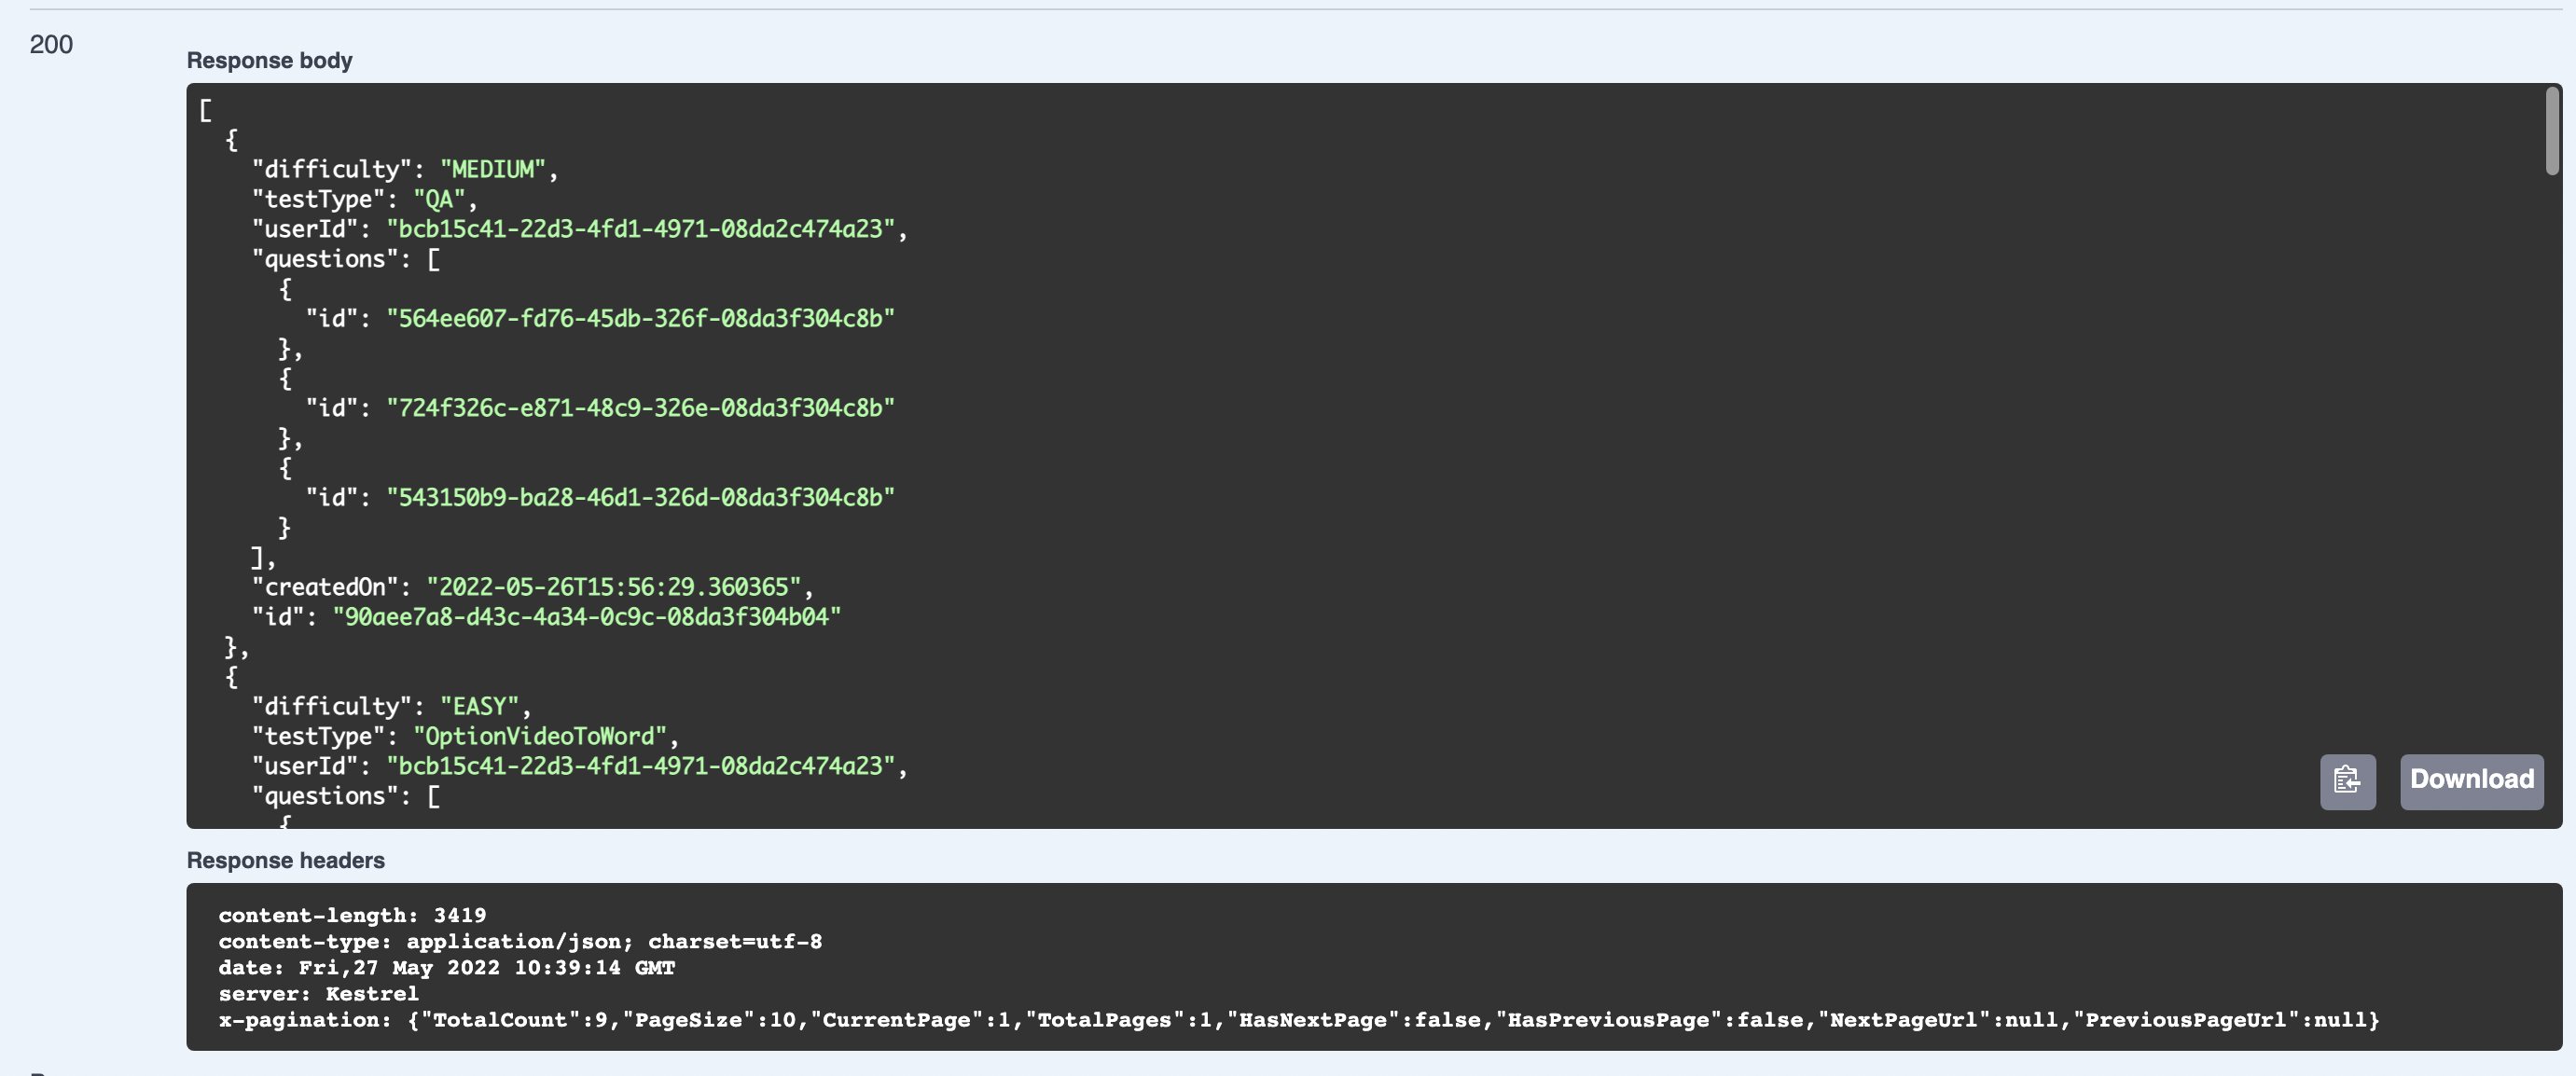
\includegraphics[width=0.9\textwidth]{assets/pagination.png}
            \caption{Paginated response}
            \label{fig:impl_pagination}
        \end{figure}

        \lstinputlisting[language=json, captionpos=t,
            caption={Metadata information about the pagination}, 
            label={lst:impl_pagination_json}]
        {code/pagination.json}
        
        \subsubsection{What is population?}
        Following the last example, imagine that I send all the information to the user about every test. The page is only displaying general information about the tests, but I'm also sending all the videos \\
        to display every test. \\
        
        As this would be very heavy, I have \textit{DTO} objects that are general. This way, I can send the general information about the test, which is the exact data the user needs. If needed more, I can "populate" the tests, this is \\
        sending all the information related to the questions.

        \begin{figure}[H]
            \centering
            \begin{subfigure}[T]{0.49\textwidth}
                \centering
                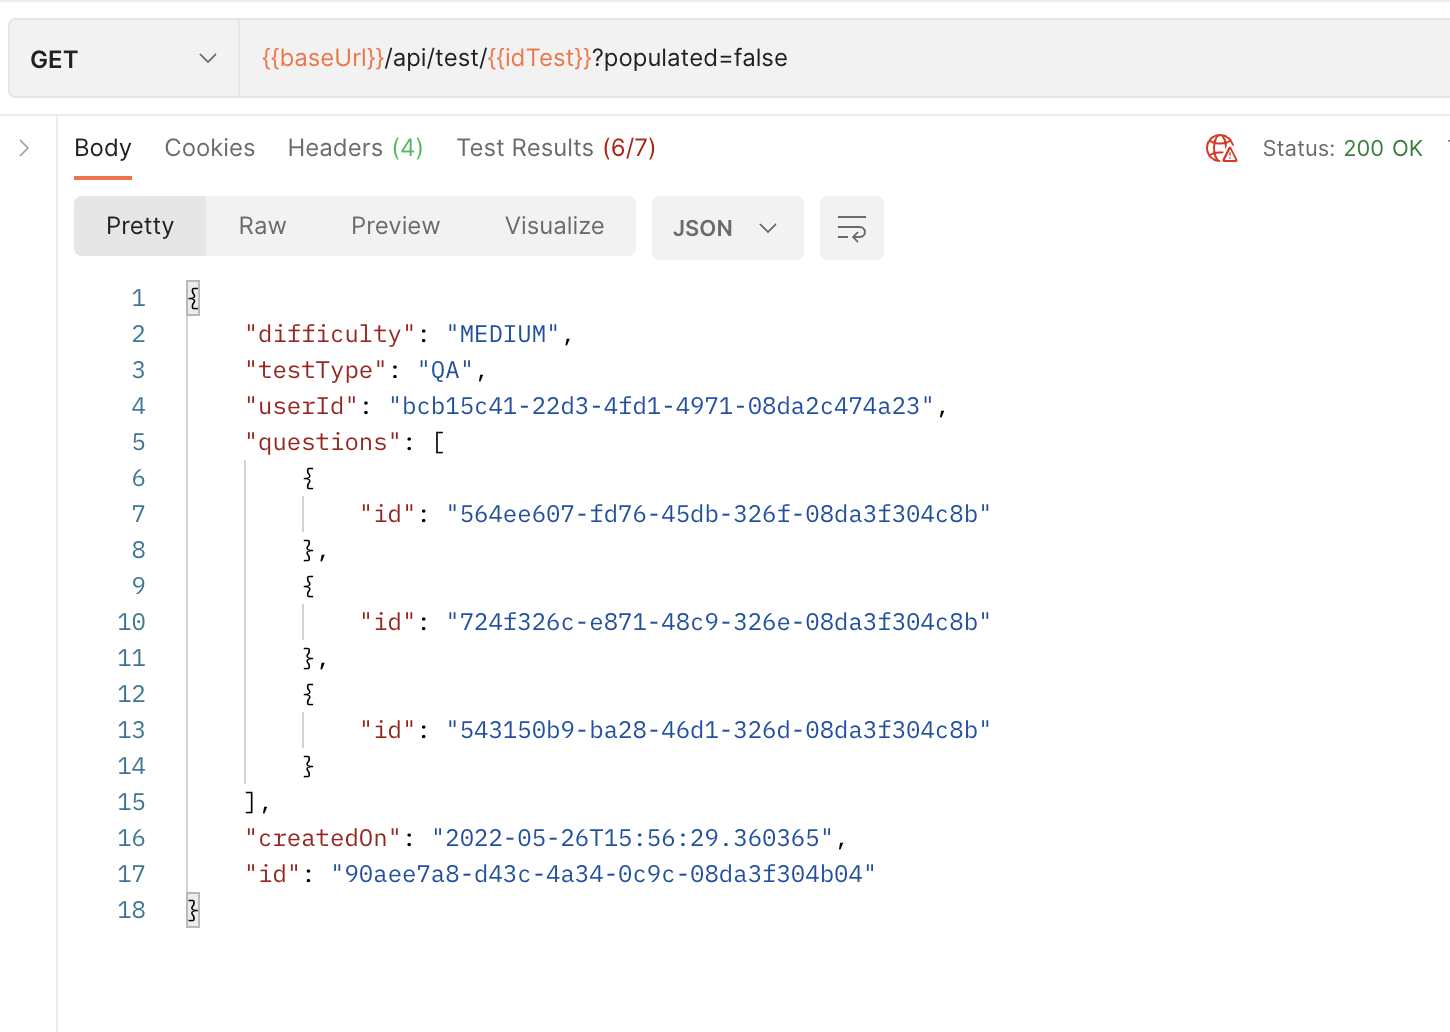
\includegraphics[width=0.48\textwidth]{assets/populated_false.png}
                \caption{Populated=false}
                \label{fig:impl_populated_false}
            \end{subfigure}
            \hfill
            \begin{subfigure}[T]{0.49\textwidth}
                \centering
                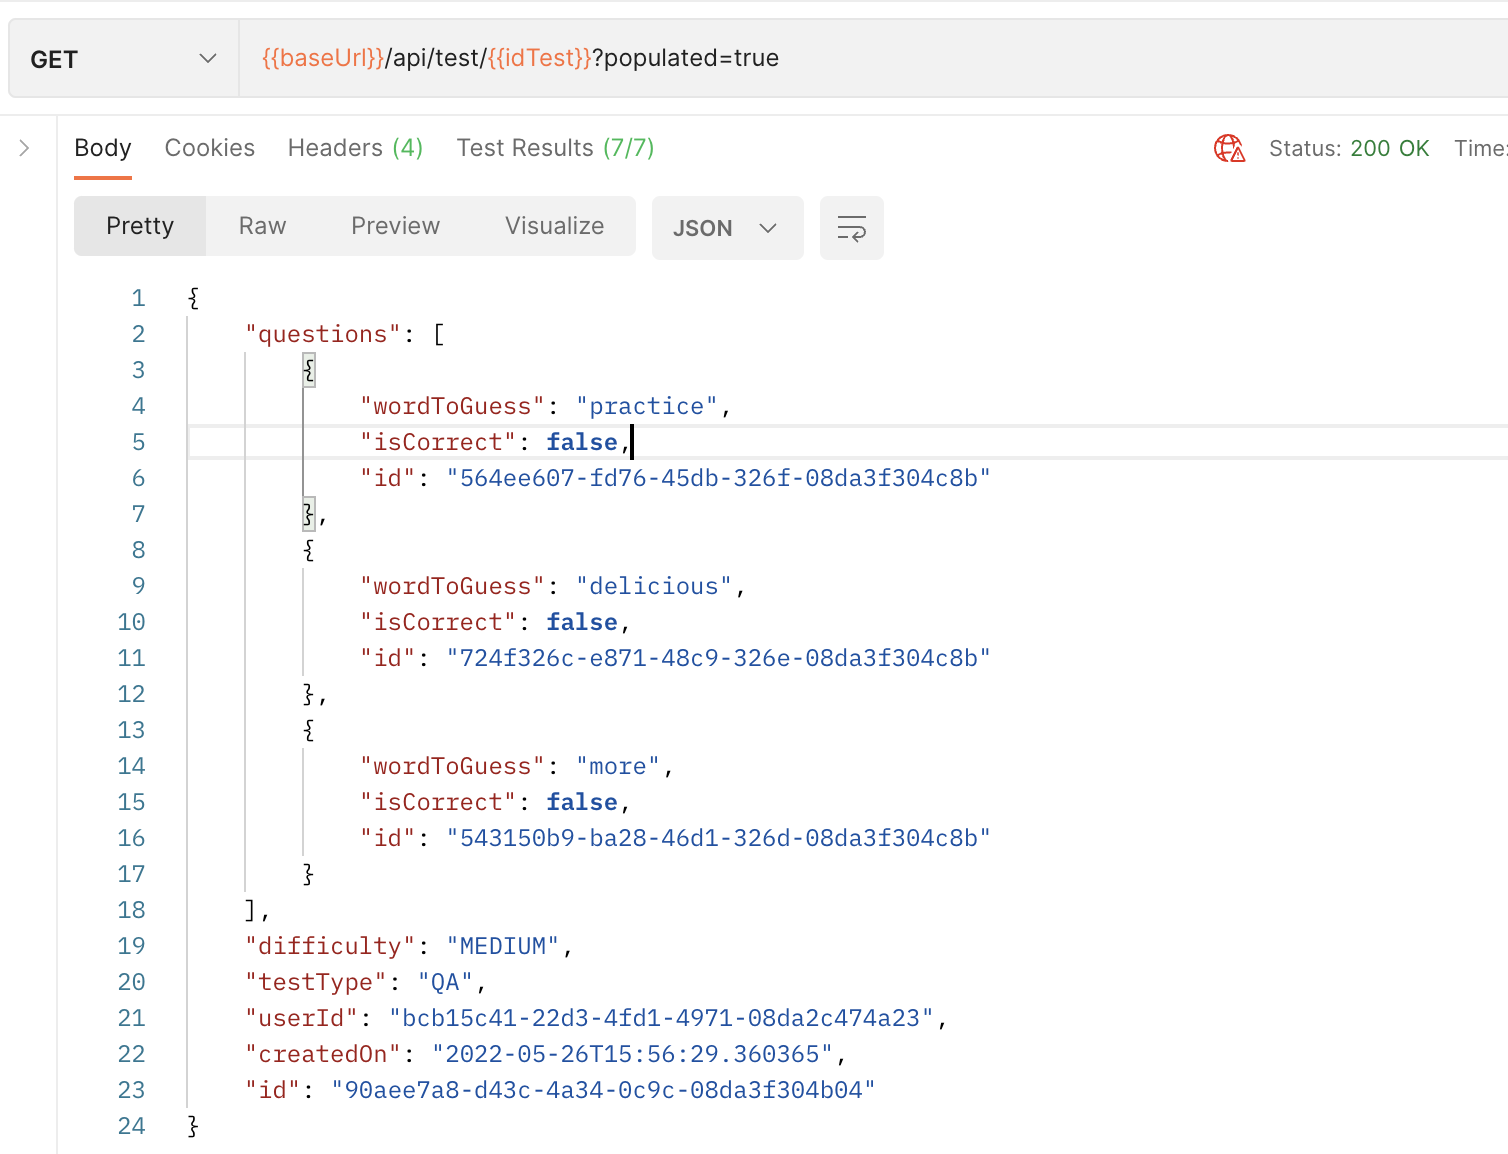
\includegraphics[width=0.48\textwidth]{assets/populated_true.png}
                \caption{Populated=true}
                \label{fig:impl_populated_true}
            \end{subfigure}
               \caption{Difference between a populated and a non-populated request}
               \label{fig:impl_populated}
        \end{figure}

    \subsection{Health check of the API}
    As Microsoft indicates \cite{Health}, it is good to add checkers for the state of the application. This way, orchestrators, logs and people can check the state of the application and its dependencies. \\
    I added a check for the application and the database context. In the next figure, you can see the difference of response got from this endpoint. \\
    
    \begin{figure}[H]
        \centering
        \begin{subfigure}[T]{0.49\textwidth}
            \centering
            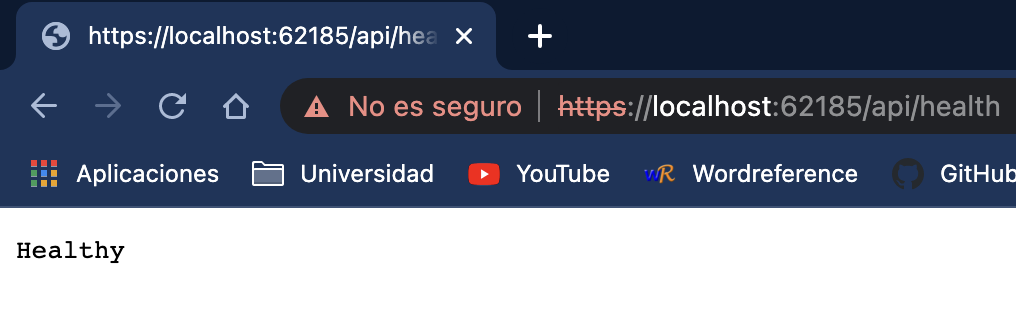
\includegraphics[width=0.48\textwidth]{assets/healthy.png}
            \caption{Healthy state}
            \label{fig:impl_healthy}
        \end{subfigure}
        \hfill
        \begin{subfigure}[T]{0.49\textwidth}
            \centering
            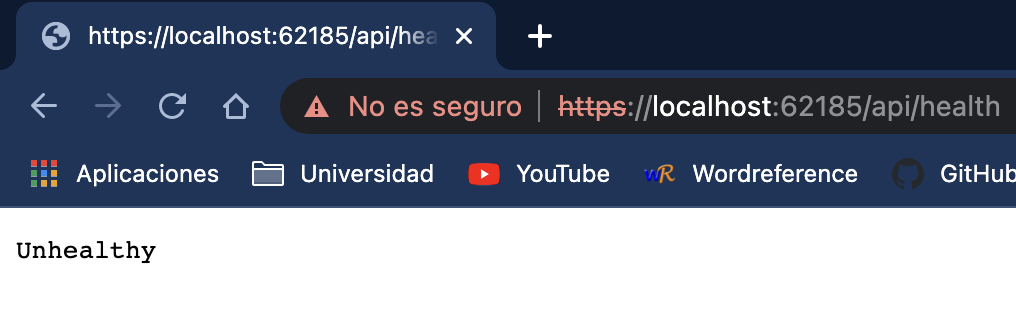
\includegraphics[width=0.48\textwidth]{assets/unhealthy.png}
            \caption{Unhealthy state}
            \label{fig:impl_unhealthy}
        \end{subfigure}
           \caption{API health checks}
           \label{fig:impl_health}
    \end{figure}

    Implement this in \textit{ASP.NET} is very easy. Just this method will do the magic. \\
    \lstinputlisting[language=CSharp, captionpos=t,
            caption={Configuring a health endpoint}, 
            label={lst:impl_health_config}]
    {code/Health.cs}

    \subsection{Documenting the API with code using Swagger}
    Swagger \cite{Swagger} is a tool to document, test and design APIs. When documenting the API with \textit{Swagger}, it creates a JSON file following the \textbf{OpenApi} specification, which allows \\
    to define an API in a language-agnostic way. Therefore, I can share this document to other apps, i.e \textit{Postman} to avoid rewriting all the endpoints.

    As it is visible in the next figure, I can document every endpoint in the API using comments. This way, my code and documentation goes together and it helps me to understand the better the functions. \\
    \begin{figure}[H]
        \centering
            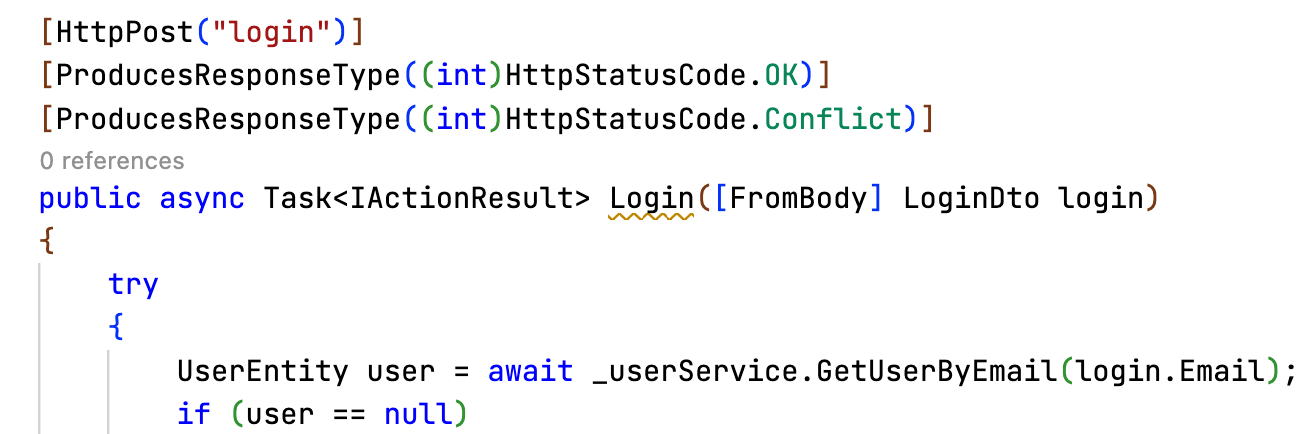
\includegraphics[width=0.9\textwidth]{assets/swagger_comment.png}
        \caption{How to document an endpoint using swagger}
        \label{fig:impl_swagger_endpoint}
    \end{figure}

    The output of documenting with Swagger the API would be this page. I can see all the endpoints of the application, execute them and see the schema definitions. This can be shared between teams and let the code as a black box. 
    \begin{figure}[H]
        \centering
            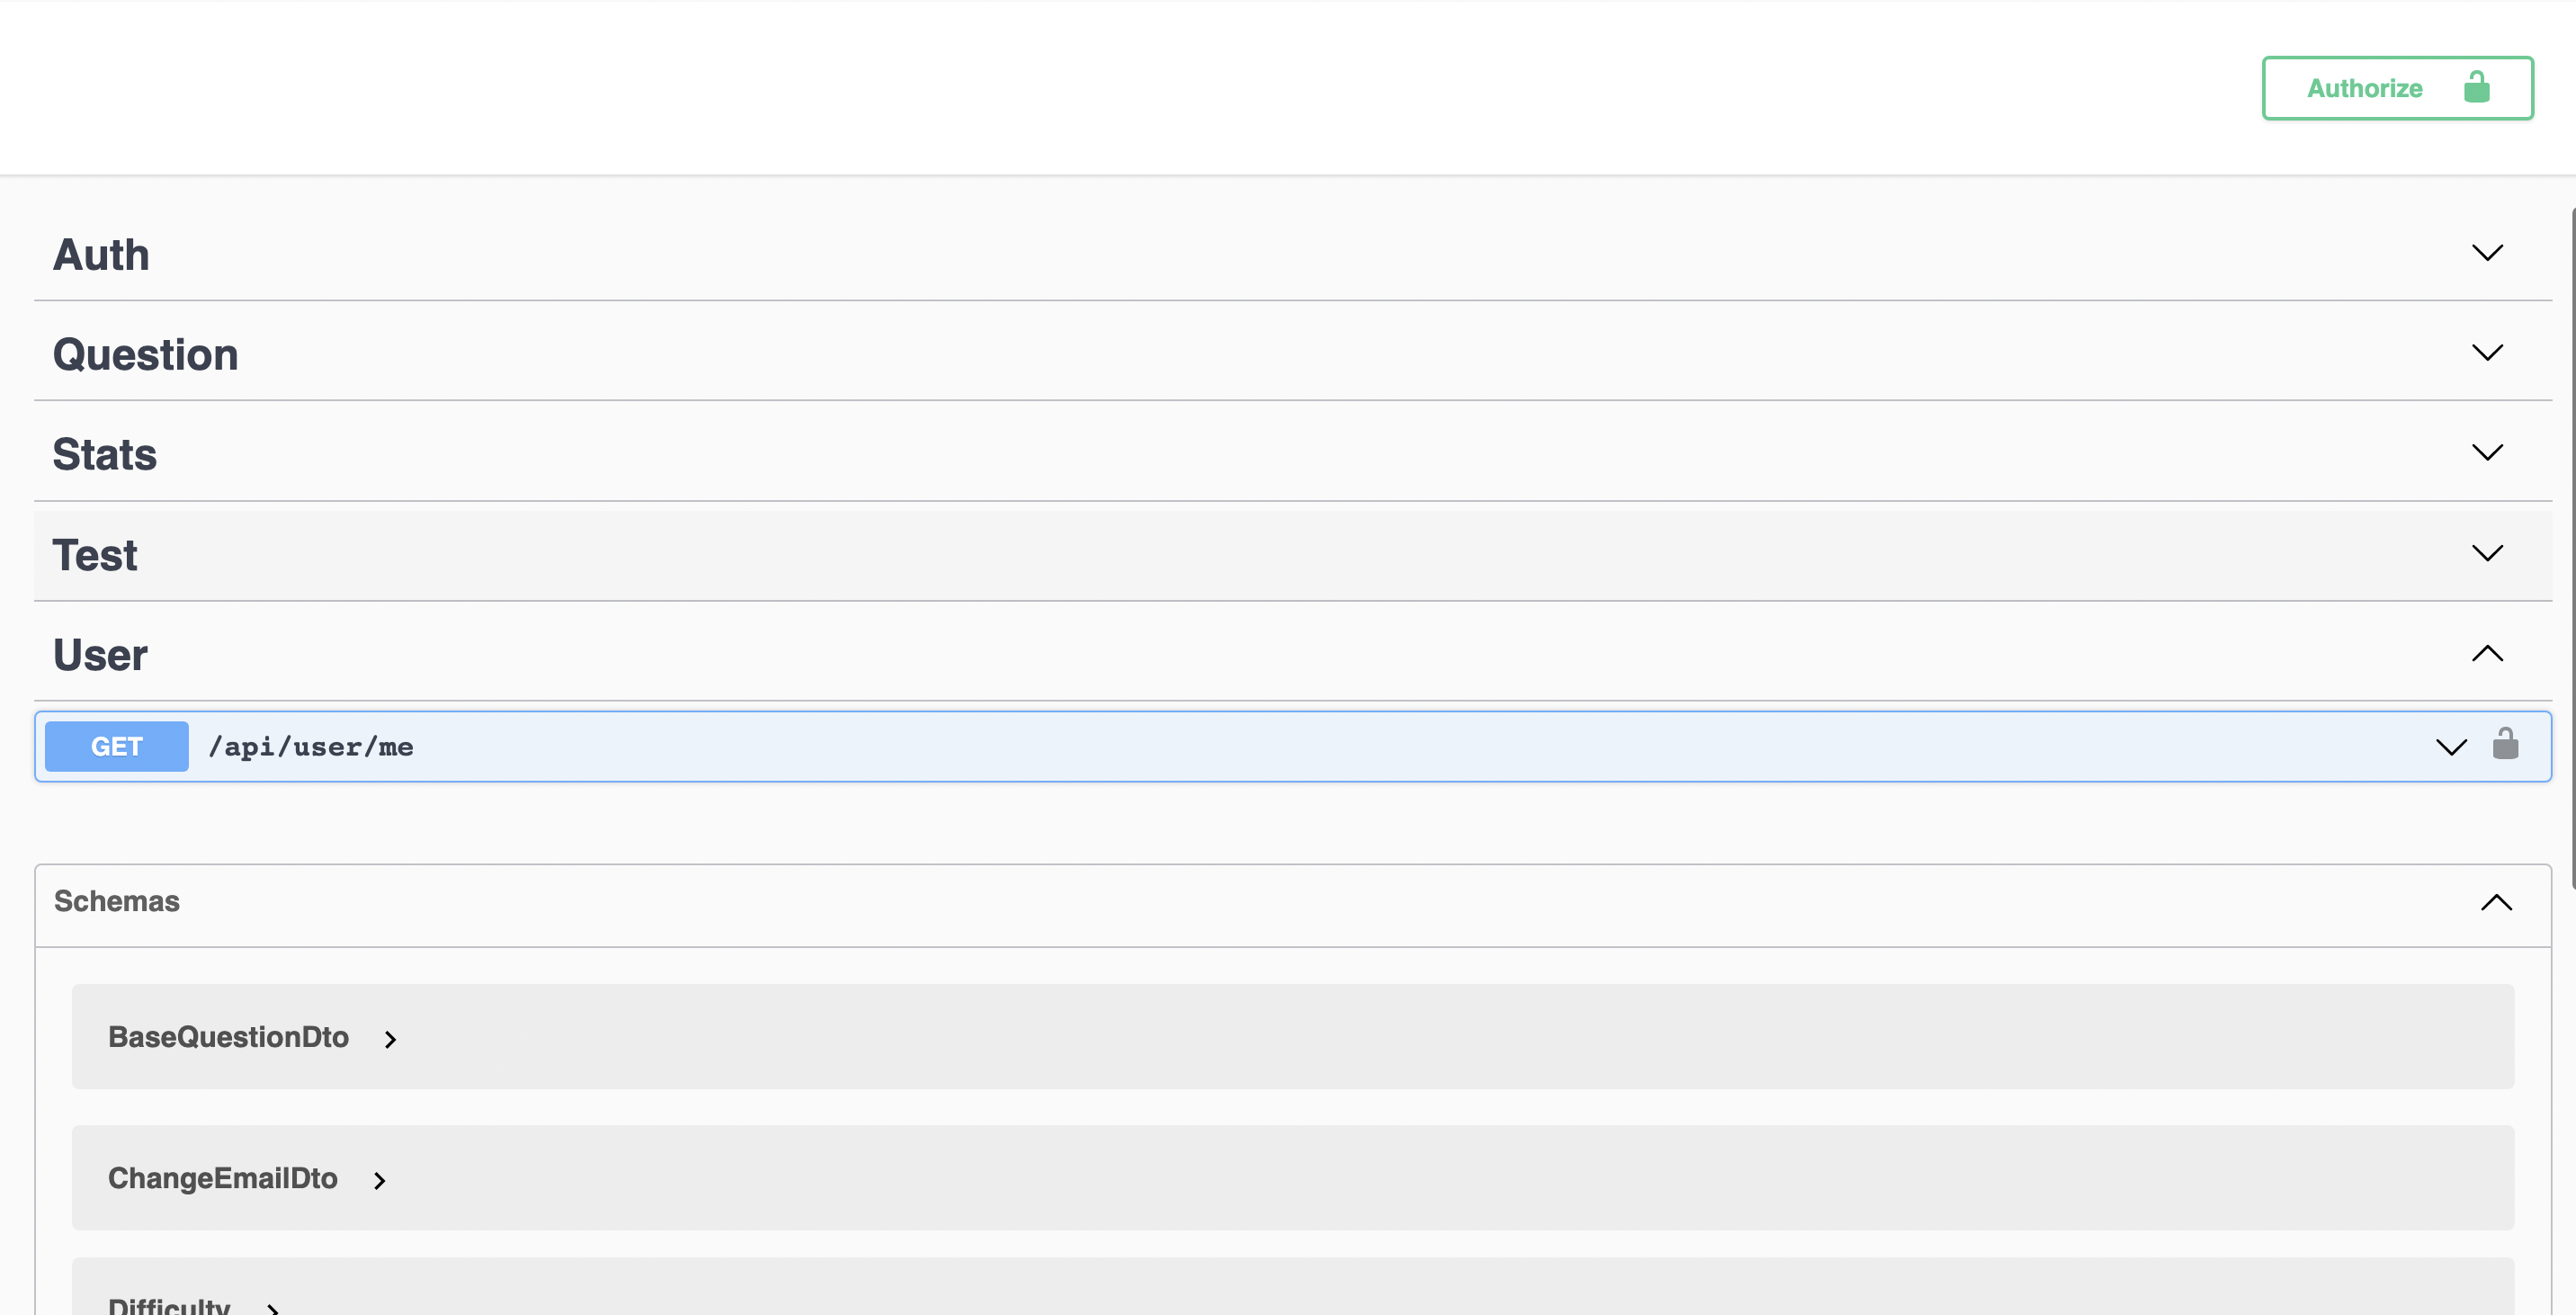
\includegraphics[width=0.9\textwidth]{assets/swagger.png}
        \caption{Swagger main page}
        \label{fig:impl_swagger}
    \end{figure}

    \subsection{Middleware diagram}
    In the next page, I included a diagram that represents the flux that a request follows from the first moment it reaches the server until the servers replies to this request. \\

    The diagram contains all the middleware layers. The ones in yellow are the ones created/configured by me. The rest are simple configured by the framework. \\

    A good explanation of this diagram should explains every middleware layer. As this is a very detailed work and unneccessary, I'll just explain a bit of every layer:
    \begin{itemize}[noitemsep]
        \item The uppest middleware layer is the \textit{Exception handler}. It is in charge of capturing the exceptions and reply correctly when something happens and log it.
        \item The \textit{Static files middleware} is in charge of give access to the filesystem. \\
        \item The \textit{CORS middleware} is in charge of configure the \textit{CORS} policy. \\
        \item The \textit{JWT middleware} is in charge of authorization and authentication. It checks the {JWT token} sent by the user in the request. 
        \item The \textit{Validation middleware} is in charge of validating the objects or fields sent in the {HTTP request}. This way, data sent incorrectly won't be processed. For instance, if the user asked for the tests done by him from tomorrow, this middleware would stop the flux as there can not be tests done from tomorrow. This query wouldn't go to the database. 
    \end{itemize}
        \newpage
        \begin{figure}[H]
            \centering
                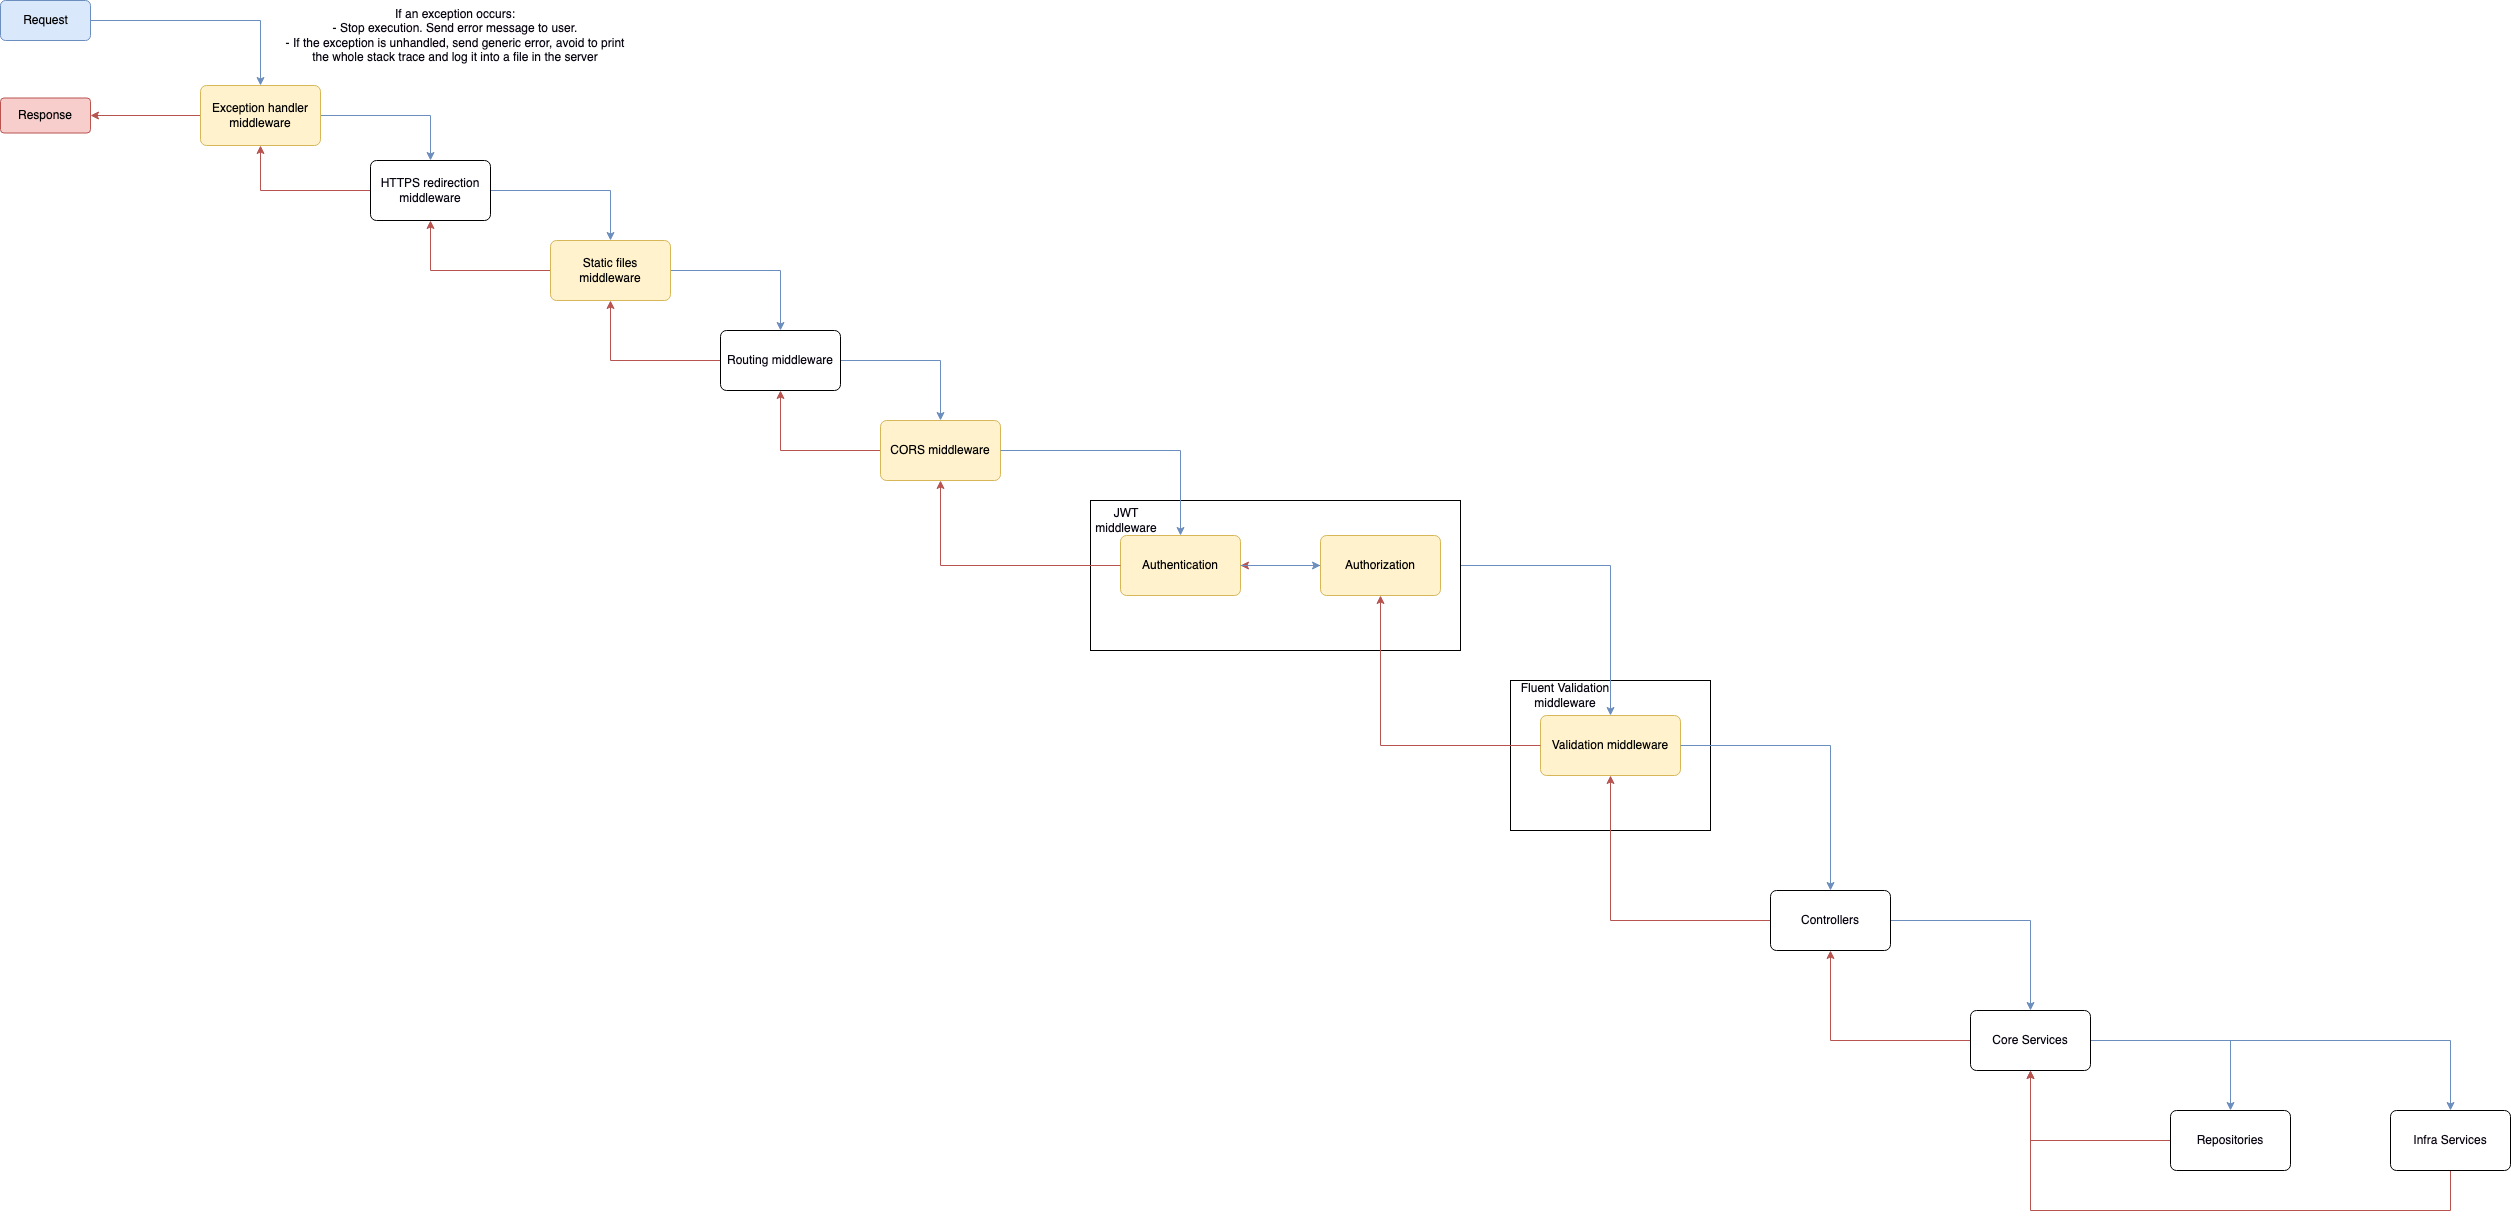
\includegraphics[angle=90, width=\textwidth, height=\textheight]{assets/diagrams/middleware.png}
            \caption{Middleware flux}
            \label{fig:implementation_middleware}
        \end{figure}

    \section{Sequence diagram, common}
    All requests have to go through the middleware flux. There are some middlewares that are common for all requests. These are the \textit{ErrorHandlingMiddleware}, \textit{ValidationMiddleware} and the \textit{AuthenticationHandler}. \\
    Once the request passes through these middlewares, it reaches the controller.
        \begin{figure}[H]
            \centering
                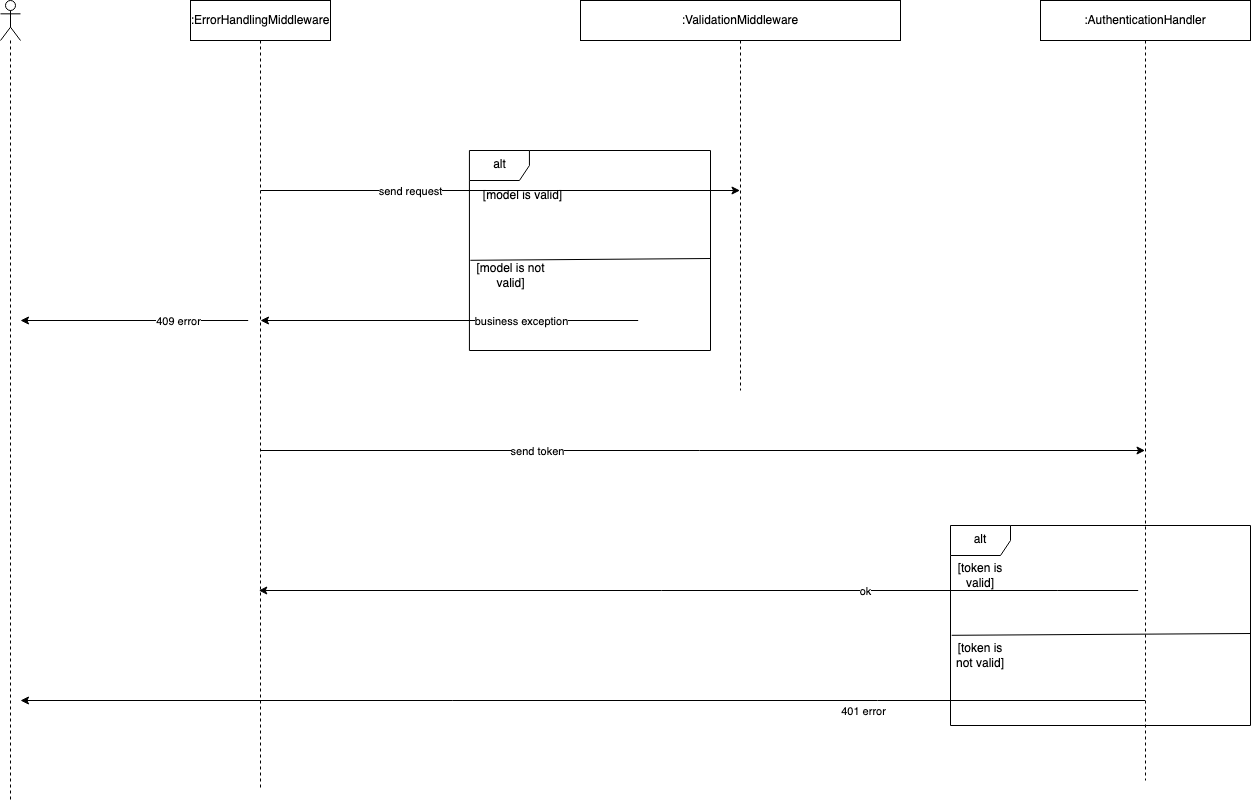
\includegraphics[width=\textwidth]{assets/diagrams/sequence_common.png}
            \caption{Common behaviour sequence diagrams}
            \label{fig:implementation_common}
        \end{figure}


    \section{Sequence diagram, use case: \textit{Delete a test}}
    The user sends a request to the api to delete a test. The API would respond ok if the test have been succesfully deleted or conflict if an error has ocurred. \\
    When the request arrives at the controller, the controller delegates in the \textit{TestService} the deletion of the test. It retrieves the test, check if the test is from the user and delete the test from the database and from the storage. \\
        \begin{figure}[H]
            \centering
                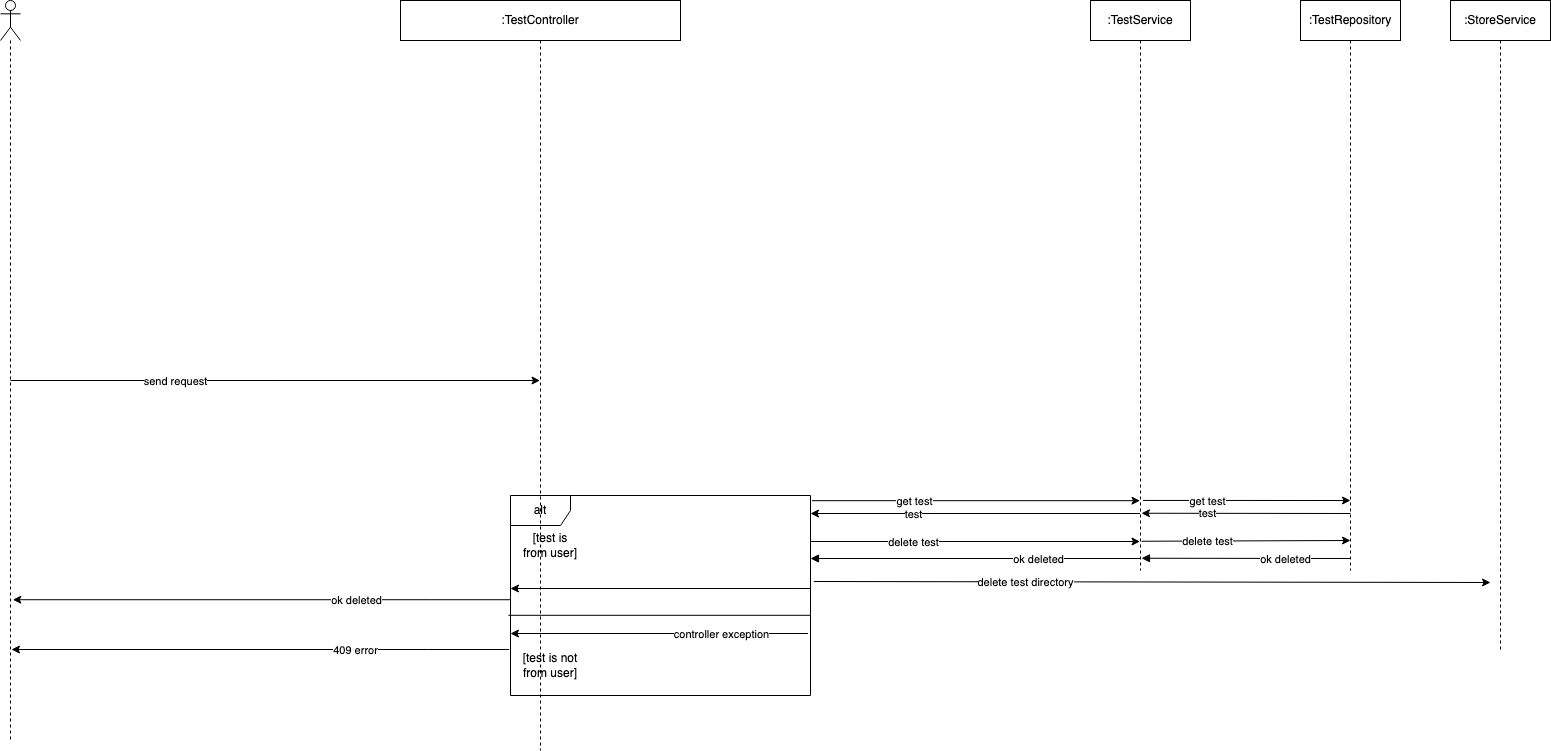
\includegraphics[width=\textwidth]{assets/diagrams/deletetest.png}
            \caption{Sequence diagram: delete a test use case}
            \label{fig:implementation_deletetest}
        \end{figure}

    \section{Complete sequence diagram, use case: \textit{Get a test}}
    This would be the complete sequence diagram, including the common part. Once the request passes all the middleware, it reaches the \textit{TestController}. It delegates the action into the \textit{TestService}. This gets the test from the repository, \\ 
    check if the user is the owner of the test and if everything is okay it returns the test to the controller to be sent to the user. \\
    If an alternative flux happens, a \textit{BusinessException} will be thrown and the user will receive an error message and code.
        \newpage
        \begin{figure}[H]
            \centering
                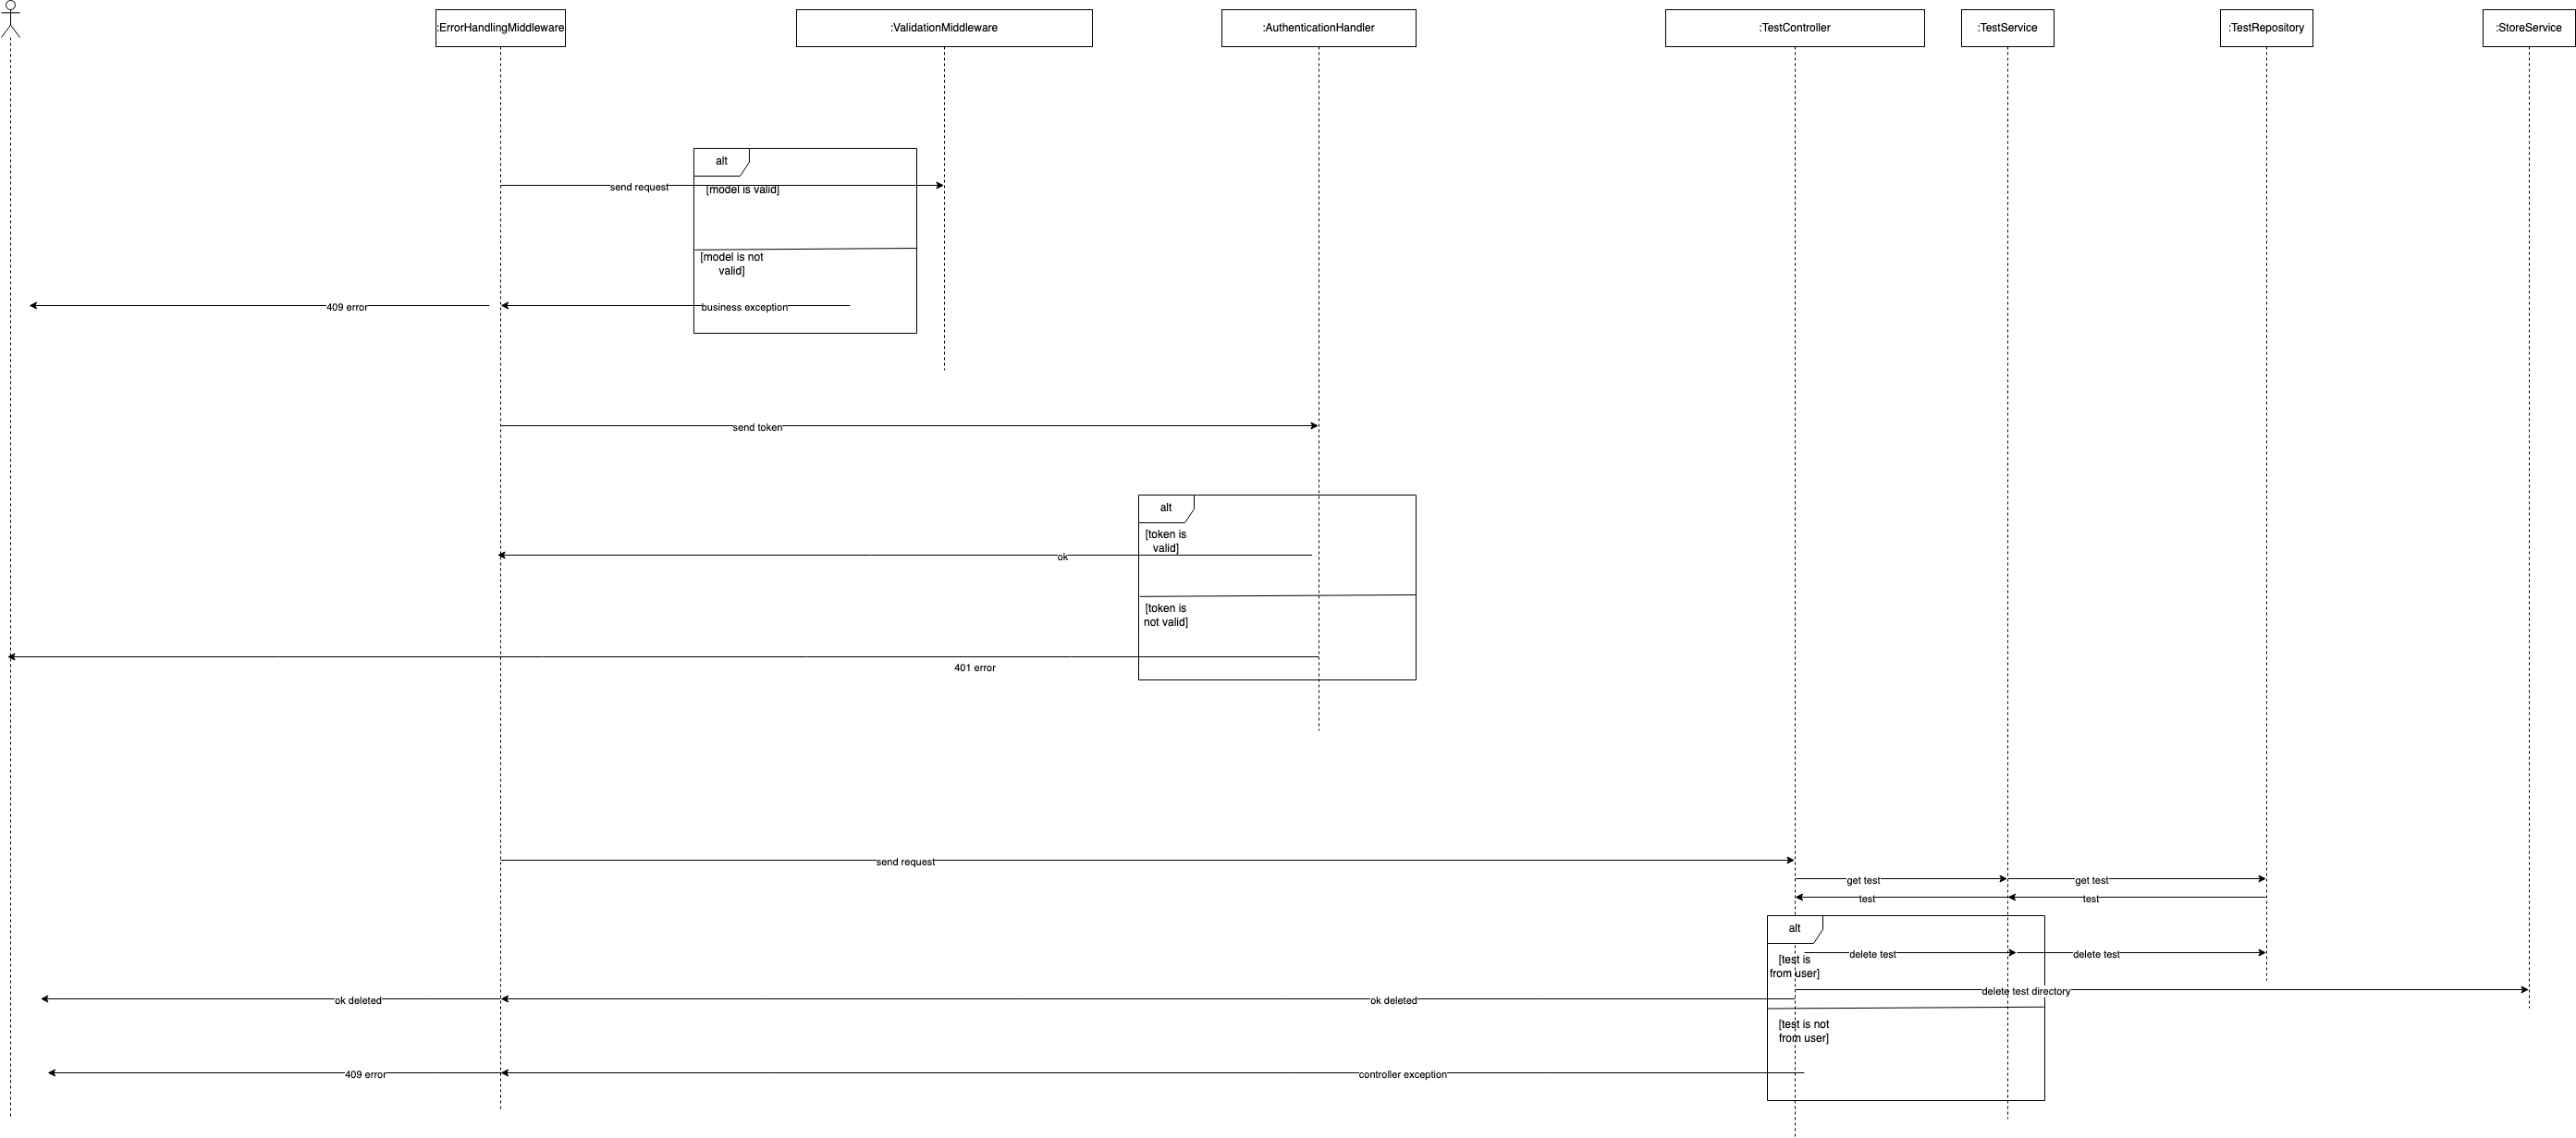
\includegraphics[angle=90, width=\textwidth, height=\textheight]{assets/diagrams/getatest.png}
            \caption{Sequence diagram: get a test use case}
            \label{fig:implementation_getatest}
        \end{figure}

\newpage
\section{Frontend code documentation}
    \subsection{Organization of the project}
    \subsection{Redux pattern}
    \subsection{Private VS public routes}
    \subsection{Intelligent forms using Formik}
        \subsubsection{Custom component to integrate Material UI and Formik}
    \subsection{Persisting the data}

\newpage
\section{AI service code documentation}
    \subsection{API keys}
    \subsection{Protecting the API using JWT}
    \subsection{Validating the videos}
    \subsection{Initializing the model}
    \subsection{Executing the model}
        \subsection{Video transformations}
    \subsection{Example}
    
